%%%%%%%%%%%%%%%%%%%%%%%%%%%%%%%%%%%%%%%%%%%%%%%%%%%%%%%%%%%%%%%%%%%%%%%%%%%%%%%%
%%
%% Para utilizar ese modelo sao necessarios os seguintes arquivos:
%%
%% copin.cls
%% copin.sty
%% mestre.sty
%%
%%%%%%%%%%%%%%%%%%%%%%%%%%%%%%%%%%%%%%%%%%%%%%%%%%%%%%%%%%%%%%%%%%%%%%%%%%%%%%%%

\documentclass[a4paper,titlepage]{sty/copin}

\usepackage[portuges,english]{babel}
\usepackage{sty/copin,sty/mestre,epsfig}
\usepackage{times}
\usepackage{url}
\usepackage{icomma}

\makeatletter
\g@addto@macro{\UrlBreaks}{\UrlOrds}
\makeatother
\usepackage{footmisc}
\usepackage{pifont}
\usepackage{xcolor}
\definecolor{britishracinggreen}{rgb}{0.0, 0.26, 0.15}
\definecolor{gray}{rgb}{0.4,0.4,0.4}
\definecolor{darkblue}{rgb}{0.0,0.0,0.6}
\definecolor{cyan}{rgb}{0.0,0.6,0.6}
\usepackage{chngcntr}
\counterwithout{footnote}{chapter}

%-------------------------- Para usar acentuacaoo em sistemas ISO8859-1 ------------------------------------
% Se estiver usando o Microsoft Windows ou linux com essa codificacao, descomente essa linhas abaixo
% e comente as linhas referentes ao UTF8
%\usepackage[latin1]{inputenc} % Usar acentuacao em sistemas ISO8859-1, comentar a linha com  \usepackage[utf8x]{inputenc}
%-----------------------------------------------------------------------------------------------------

%-------------------------- Para usar acentuacao em sistemas UTF8 ------------------------------------
% Para a maior parte das distribuicoes linux, usar a opcao utf8x (lembrar de comentar as linha referente a ISO8859-1 acima)
\usepackage{ucs}
\usepackage[utf8x]{inputenc}
%\usepackage[utf8]{inputenc}
\usepackage[T1]{fontenc}
%-----------------------------------------------------------------------------------------------------


\usepackage{fancyhdr}
\usepackage{graphicx}
\graphicspath{{img/}}
\DeclareGraphicsExtensions{.pdf,.jpeg,.png,.eps}
\usepackage[caption=false,font=footnotesize,labelfont=sf,textfont=sf]{subfig}
\usepackage{longtable} %tabelas longas, para tabelas que ultrapassam uma pagina
%\input{psfig.sty}
\usepackage{pdfpages}


% ----------------- Para inserir codigo fonte de linguagens de programacao no documento -------------
\usepackage{listings}
\lstset{language=C,
	breaklines=true,
    xleftmargin=9pt,
    basicstyle=\ttfamily\footnotesize,
    keywordstyle=\color{olive}\bfseries\ttfamily,
    stringstyle=\color{red}\ttfamily,
    commentstyle=\color{britishracinggreen}\ttfamily,
    morecomment=[l][\color{magenta}]{\#},
    directivestyle={\color{RawSienna}},
    numbers=left, % where to put the line-numbers
    numberstyle=\scriptsize,
    backgroundcolor=\color{white},
    emph={uint8_t},emphstyle={\color{olive}\bfseries\ttfamily},
	showstringspaces=false,
	firstnumber=1,
    extendedchars=true,
    inputencoding=utf8x,
	frame=tb
}

\lstset{language=XML,
  basicstyle=\ttfamily,
  columns=fullflexible,
  showstringspaces=false,
  commentstyle=\color{gray}\upshape
}

\lstdefinelanguage{XML}
{
  morestring=[b]",
  morestring=[s]{>}{<},
  morecomment=[s]{<?}{?>},
  stringstyle=\color{black},
  identifierstyle=\color{darkblue},
  keywordstyle=\color{cyan},
  morekeywords={xmlns,version,type}% list your attributes here
}

\lstdefinelanguage
   [x64]{Assembler}     % add a "x64" dialect of Assembler
   [x86masm]{Assembler} % based on the "x86masm" dialect
   % with these extra keywords:
   {morekeywords={CDQE,CQO,CMPSQ,CMPXCHG16B,JRCXZ,LODSQ,MOVSXD, %
                  POPFQ,PUSHFQ,SCASQ,STOSQ,IRETQ,RDTSCP,SWAPGS,retq} %
                  %rax,rdx,rcx,rbx,rsi,rdi,rsp,rbp, %
                  %r8,r8d,r8w,r8b,r9,r9d,r9w,r9b} %
                  } % etc.

\lstset{language=[x64]Assembler,
    breaklines=true,
    xleftmargin=9pt,
    basicstyle=\ttfamily\footnotesize,
    keywordstyle=\color{olive}\bfseries\ttfamily,
    stringstyle=\color{red}\ttfamily,
    commentstyle=\color{britishracinggreen}\ttfamily,
    morecomment=[l][\color{magenta}]{\#},
    directivestyle={\color{RawSienna}},
    numbers=left, % where to put the line-numbers
    numberstyle=\scriptsize,
    backgroundcolor=\color{white},
    showstringspaces=false,
    extendedchars=true,
    inputencoding=utf8x,
    keywords={push, mov, add, pop, retq}
}

\lstset{literate={á}{{\'{a}}}1 {é}{{\'{e}}}1 {í}{{\'{i}}}1 {ó}{{\'{o}}}1 {ú}{{\'{u}}}1 {ç}{{\c{c}}}1 {à}{{\`{a}}}1 {â}{{\^{a}}}1 {ê}{{\^{e}}}1 {ô}{{\^{o}}}1 {ã}{{\~{a}}}1 {õ}{{\~{o}}}1}

\renewcommand{\lstlistingname}{Código Fonte}
\renewcommand{\lstlistlistingname}{Lista de Códigos Fonte}
\newcommand\fixme[1]{\textcolor{red}{#1}}
\newcommand\comment[1]{\textcolor{blue}{#1}}
% ---------------------------------------------------------------------------------------------------

\selectlanguage{portuges}
\sloppy

\begin{document}

%%%%%%%%%%%%%%%%%%%%%%%%%%%%%%%%%%%%%%%%%%%%%%%%%%%%%%%%%%%%%%%%%%%%%%%%%%%%%%%%
\Titulo{Desafios no Desenvolvimento de Aplicações\\Seguras Usando Intel SGX}
\Autor{Rodolfo de Andrade Marinho Silva}
\Data{01 de março de 2018}
\Area{Ciência da Computação}
\Pesquisa{Segurança da Informação}
\Orientadores{Andrey Elísio Monteiro Brito  \\
	 (Orientador)}

\newpage
\cleardoublepage

\PaginadeRosto

\newpage
\cleardoublepage

%%%%%%%%%%%%%%%%%%%%%%%%%%%%%%%%%%%%%%%%%%%%%%%%%%%%%%%%%%%%%%%%%%%%%%%%%%%%%%%%
\begin{resumo} 
No decorrer das últimas décadas, uma quantidade de dados de usuários cada vez
maior vem sendo enviada para ambientes não controlados pelos mesmos. Em alguns
casos esses dados são enviados com o objetivo de tornar esses dados públicos,
mas na grande maioria das vezes há a necessidade de manter esses dados seguros e
privados, ou autorizar o seu acesso apenas em usos bem específicos. Considerando
o caso onde os dados devem ser mantidos privados, entidades devem tomar cuidados
especiais para manter a segurança e privacidade de tais dados tanto durante a
transmissão quanto durante o armazenamento e processamento dos mesmos. Com esse
objetivo, vários esforços vêm sendo feitos, inclusive o desenvolvimento de
componentes de \textit{hardware} que provêem ambientes de execução confiável,
\textit{TEEs}, como o \textit{Intel Software Guard Extensions} (\textit{SGX}).
O uso dessa tecnologia, porém, pode ser feito de forma incorreta ou ineficiente,
devido a cuidados não observados durante o desenvolvimento de aplicações.

O trabalho apresentado nessa dissertação aborda os principais desafios
enfrentados no desenvolvimento de aplicações que façam uso de \textit{SGX}, e
propõe boas práticas e um conjunto de ferramentas (\textit{DynSGX}) que ajudam
a fazer melhor uso das capacidades da tecnologia. Tais desafios incluem, mas não
são limitados a, particionamento de aplicações de acordo com o modelo de
programação do SGX, colocação de aplicações em ambientes de computação na nuvem,
e, sobretudo, gerência de memória.

Os estudos apresentados neste trabalho apontam que o mal uso da tecnologia pode
acarretar em uma perda de performance considerável se comparado com
implementações que levam em conta as boas práticas propostas. O conjunto de
ferramentas proposto neste trabalho também mostrou possibilitar a proteção de
código de aplicações em ambientes de computação na nuvem, com uma sobrecarga
desprezível em comparação com o modelo de programação padrão de SGX.
\end{resumo}

\newpage
\cleardoublepage

%%%%%%%%%%%%%%%%%%%%%%%%%%%%%%%%%%%%%%%%%%%%%%%%%%%%%%%%%%%%%%%%%%%%%%%%%%%%%%%%
\begin{summary}
During the last few decades, an increasing amount of user data have been sent
to environments not controlled by data owners. In some cases these data are sent with
the objective to turn them public, but in the vast majority of times, these data
need to be kept safe and private, or to be allowed access only in very specific
use cases. Considering the case where data need to be kept private, entities
must take specific measures to maintain the data security and privacy while
transmitting, storing and processing them. With this objective many efforts
have been made, including the specification of hardware components that provide
a trusted execution environment (TEEs), like the Intel Software Guard Extensions
(SGX). The use of this technology , though, can be made in incorrect or
ineffective ways, due to not taking some considerations into account during the
development of applications.

In this work, we approach the main challenges faced in the development of
applications that use SGX, and propose good practices and a toolset (DynSGX)
that help making better use of the capabilities of this technology. Such
challenges include, but are not limited to, application partitioning,
application colocation in cloud computing environments, and memory management.

The studies presented in this work show that the bad use of this technology can
result in a considerable performance loss when compared to
implementations that take into account the good practices proposed. The toolset
proposed in this work also showed to enable protecting application code in cloud
computing environments, having a negligible performance overhead when
compared to the regular SGX programming model.
\end{summary}

\newpage
\cleardoublepage

%%%%%%%%%%%%%%%%%%%%%%%%%%%%%%%%%%%%%%%%%%%%%%%%%%%%%%%%%%%%%%%%%%%%%%%%%%%%%%%%
\begin{agradecimentos}
Primeiramente, a Deus, agradeço pelos dons recebidos, que me possibilitaram
pensar e desenvolver este trabalho de pesquisa.

Agradeço à minha família pelo apoio e incentivo à minha formação, dados durante toda a minha vida.

A Elaine, pelo companheirismo e paciência em momentos cruciais no decorrer do
mestrado, especialmente durante a reta final.

Agradeço também ao LSD, pelos agradáveis ambiente e infraestrutura providos, e
pela grande interdisciplinaridade de projetos existentes, que contribuíram para
enxergar como meu trabalho se insere no mundo real.

Aos amigos do projeto SecureCloud (Marcus, Lília, Gabriel, Amanda, Fábio,
Leandro, Pedro, Dalton, Matteus, Jefferson, Ionésio e Léo), agradeço por
colaborarem diretamente com o desenvolvimento deste mestrado, seja provendo
algumas dúvidas, seja provendo soluções para outras dúvidas, e aos demais
companheiros de sala (Igor, Iury, Roberto, e Armstrong) pelas discussões sobre
os mais variados temas, necessárias para refrescar um pouco a mente após longos
períodos de estudo.

Por fim, mas não menos importante, agradeço a meu orientador, Andrey, pelos
conselhos dados, pela confiança em meu trabalho, e, sobretudo, pela constante
empolgação com o tema sendo pesquisado.

A todos vocês, o meu muito obrigado!
\end{agradecimentos}

\clearpage

%%%%%%%%%%%%%%%%%%%%%%%%%%%%%%%%%%%%%%%%%%%%%%%%%%%%%%%%%%%%%%%%%%%%%%%%%%%%%%%%
%% Definicao do cabecalho: secao do lado esquerdo e numero da pagina do lado direito
\pagestyle{fancy}
\addtolength{\headwidth}{\marginparsep}\addtolength{\headwidth}{\marginparwidth}\headwidth = \textwidth
\renewcommand{\chaptermark}[1]{\markboth{#1}{}}
\renewcommand{\sectionmark}[1]{\markright{\thesection\ #1}}\lhead[\fancyplain{}{\bfseries\thepage}]%
	     {\fancyplain{}{\emph{\rightmark}}}\rhead[\fancyplain{}{\bfseries\leftmark}]%
             {\fancyplain{}{\bfseries\thepage}}\cfoot{}

%%%%%%%%%%%%%%%%%%%%%%%%%%%%%%%%%%%%%%%%%%%%%%%%%%%%%%%%%%%%%%%%%%%%%%%%%%%%%%%%
\selectlanguage{portuges}

\Sumario
\ListadeSimbolos
\listoffigures
\listoftables
\lstlistoflistings %lista de codigos fonte - Para inserir a listagem de codigos fonte
\newpage
\cleardoublepage

\Introducao


%%%%%%%%%%%%%%%%%%%%%%%%%%%%%%%%%%%%%%%%%%%%%%%%%%%%%%%%%%%%%%%%%%%%%%%%%%%%%%%%
%
% Hifenizacao - Colocar lista de palavras que nao devem ser separadas e que 
% nao estao no dicionario portugues.
% As palavras do dicionario portugues ja sao separadas corretamente pelo lateX
%
\hyphenation{ Hardware Software Intel recursive etc }

%%%%%%%%%%%%%%%%%%%%%%%%%%%%%%%%%%%%%%%%%%%%%%%%%%%%%%%%%%%%%%%%%%%%%%%%%%%%%%%%
%% A partir daqui coloque seus capitulos. Sugere-se que eles sejam inseridos com o comando \input
%% Da seguinte maneira:
%%
%% \input{cap1} 
%% \input{cap2}
% \chapter{TODO}
\fixme{
\begin{itemize}
    \item Abordagem
    \begin{itemize}
        \item Colocação de aplicações
        \item Primitivas criptográficas
    \end{itemize}
    \item Apêndice: desenvolvimento de aplicação DynSGX
\end{itemize}
}
\chapter{Introdução}
\label{chapter:intro}

\section{Contextualização}
\label{sec:intro_contextualizacao}

\subsection{Segurança e privacidade}
\label{subsec:intro_contextualizacao_seguranca_privacidade}

Vivemos em um mundo que está a cada dia mais conectado, onde pessoas estão
constantemente enviando dados pessoais para ambientes que não podem ser
controlados por elas. Ocasionalmente, esses dados são destinados a tornarem-se
públicos. Na maioria dos casos, porém, eles devem ser mantidos privados e/ou
seguros -- tais dados serão doravante denominados \textbf{dados sensíveis}.
Nesse sentido, desenvolvedores de aplicações devem encontrar formas de proteger
os dados de seus usuários contra roubo ou modificações indevidas a todo custo.

Além disso, desenvolvedores e empresas frequentemente hospedam suas aplicações
em ambientes de nuvem pública, com o objetivo de aumentar sua disponibilidade e
escalabilidade, ou até mesmo para diminuir os custos com infraestrutura física
\cite{armbrust2010view}. Em tais ambientes, múltiplas aplicações de diferentes
donos podem residir no mesmo servidor físico, possibilitando que usuários
maliciosos explorem vulnerabilidades de segurança existentes para obter dados
sensíveis de outros usuários.

Para  entender os requisitos de aplicações que lidam com dados sensíveis em
cenários como os supracitados, precisamos primeiramente definir os conceitos de
segurança e privacidade. Segurança diz respeito a proteções contra acesso,
modificação e remoção de dados sensíveis por pessoas não autorizadas.
Privacidade, por sua vez, diz repeito à proteção contra o uso de dados
sensíveis para propósitos não autorizados.

Considerando esses conceitos, aplicações que lidam com dados sensíveis devem
considerar os seguintes requisitos:

\begin{itemize}
    \item Confidencialidade -- impedir o acesso a dados sensíveis por pessoas
    não autorizadas;
    \item Disponibilidade -- garantir que dados sensíveis possam ser recuperados
    por pessoas autorizadas sempre que requisitados;
    \item Integridade -- impedir a modificação de dados sensíveis por pessoas
    não autorizadas;
    \item Privacidade -- impedir o uso de dados sensíveis para propósitos não
    autorizados.
\end{itemize}

Há situações em que desenvolvedores também desejam manter o código de suas
aplicações privado e seguro, seja pelo uso de código proprietário ou por algum
outro motivo qualquer. Nessas situações, o código de suas aplicações devem ser
tratados como dados sensíveis.

\subsection{Ambiente de execução confiável}
\label{subsec:intro_contextualizacao_tee}

O crescente volume de dados sensíveis sendo enviados, armazenados e processados
em ambientes de computação na nuvem, por um número cada vez maior de
dispositivos móveis, e as demandas de segurança e privacidade de tais dados
levaram um fórum de operadores de redes móveis (OMTP, do inglês \textit{Open
Mobile Terminal Platform}) a definir um padrão para um ambiente de execução
confiável (TEE, do inglês \textit{Trusted Execution Environment}).

Inicialmente, um TEE foi definido pela OMTP como um conjunto de componentes de
\textit{hardware} e \textit{software} que facilitam o suporte de aplicações que
satisfaçam os requisitos de um dos dois níveis de segurança definidos pela
mesma. O primeiro nível de segurança prevê proteção apenas contra ataques de
\textit{software}, enquanto o segundo nível de segurança prevê proteção contra
ataques de \textit{hardware} e de \textit{software}~\cite{omtpadvanced2009}.

Atualmente, o padrão TEE é definido pela \textit{GlobalPlatform}, uma associação
industrial que visa desenvolver padrões para processamento seguro e confiável
em serviços digitais e outros dispositivos. A \textit{GlobalPlatform} define TEE
como uma área segura do processador principal em um \textit{smart phone} ou
qualquer dispositivo conectado a ele. O TEE garante que dados sensíveis são
armazenados, processados e protegidos em um ambiente isolado e confiável~\cite
{globalplatform2017}.

De forma a facilitar o desenvolvimento de serviços que garantam segurança e
privacidade de dados sensíveis, várias implementações de TEE foram feitas~\cite
{omtpadvanced2009,logictrusted,trustonic2017,mccune2008flicker,amdSMESEV}, entre
as quais destacamos o Intel SGX, do inglês \textit{Software Guard eXtensions},
objeto de estudo deste trabalho de mestrado.

\subsection{Intel SGX}
\label{subsec:intro_contextualizacao_intel_sgx}

Com o passar do tempo, não só dispositivos móveis necessitavam de um TEE, mas
sim todo um nicho de dispositivos que lidam com dados sensíveis. Um exemplo
desses dispositivos são os computadores, sejam eles servidores usados em
ambientes de computação na nuvem, sejam eles máquinas usadas por clientes.
Visando este tipo de dispositivos, em 2013 a Intel definiu uma implementação
própria de TEE conhecida como SGX.

%%%TODO: eu preferiria mencionar por extenso dentro da seção que fala sobre ele.

Intel SGX é um conjunto de instruções incorporado às arquiteturas Intel 64 e
IA-32 que permite a criação de contêineres baseados em \textit{hardware},
chamados \textbf{enclaves}. Dados sensíveis que sejam carregados em um enclave são
protegidos contra modificação ou acesso não autorizado; Código de aplicações que
executem dentro de enclaves SGX são protegidos contra modificação~\cite
{mckeen2013innovative}.

Intel SGX está disponível em processadores da 6\textsuperscript{a} geração da
família Intel Core i, com arquitetura \textit{Skylake}, ou processadores mais
novos da mesma família, bem como em processadores da família Xeon, a partir da 5\textsuperscript{a} versão. Tais processadores estão disponíveis no mercado desde o segundo semestre do ano de  2015.

Atualmente muitas pesquisas vêm sendo desenvolvidas e publicadas\footnote{\url{https://software.intel.com/en-us/sgx/academic-research}} sobre a
aplicação de Intel SGX no mundo real~\cite{hoekstra2013using}, bem como
vulnerabilidades encontradas na tecnologia, e ações necessárias para mitigar estas vulnerabilidades~\cite{swami2017intel}.

Por ser uma tecnologia bastante promissora e já estar presente em um grande
número de processadores atualmente em uso, iremos utilizá-la como objeto de
estudo neste trabalho de dissertação.

\section{Problema investigado}
\label{sec:intro_problema_investigado}

No ano de 2016, estimou-se que o custo anual com crimes cibernéticos em alguns
países chega a um total de $USD\ 74$ milhões (setenta e quatro milhões de
dólares americanos)~\cite{costcybercrime2016}. Além disso, com a crescente produção de
dados sensíveis enviados para ambientes de computação na nuvem, cresce também a
quantidade de ataques cibernéticos com o intuito de obter e usar tais dados de
forma não autorizada. Levando em consideração esses fatos, desenvolvedores de
aplicações que lidam com dados sensíveis devem cada vez mais procurar formas de
garantir a segurança e a privacidade dos dados de seus clientes.

Uma forma de proteger os dados de usuários é através do uso de um TEE. Uma das
implementações de um TEE, que está cada vez mais difundida em máquinas de
usuários e em máquinas servidoras de computação na nuvem, é o Intel SGX. Assim
como qualquer outra tecnologia, Intel SGX também possui vulnerabilidades, como
falta de proteção contra ataques de canal lateral, que podem impactar as
garantias de segurança providas por aplicações que façam uso da tecnologia, bem
como limitações, como um pequeno espaço de memória disponível, que podem
impactar o desempenho dessas aplicações devido ao seu mau uso.

Para tirar o melhor proveito de Intel SGX, desenvolvedores devem tomar várias
decisões na hora de desenvolver suas aplicações, como: $(i)$ qual porção da
aplicação realmente precisa ser protegido pelas instruções do SGX, $(ii)$ como
gerenciar a memória consumida por suas aplicações, e $(iii)$ como evitar ataques
de canal lateral.

\section{Contribuições e relevância}
\label{sec:intro_contribuicoes}

Este trabalho tem como objetivo abordar os problemas de vulnerabilidades e baixa
eficiência de aplicações, oriundos de más práticas no uso de Intel SGX,
investigando arquitetura, implementação e implantação de aplicações que façam
uso dessa tecnologia. Com esse objetivo, são propostas várias práticas que devem
ser consideradas durante o processo de desenvolvimento de aplicações que lidam
com dados sensíveis. Tais práticas levam em consideração as vulnerabilidades e
limitações do Intel SGX, bem como o ambiente onde essas aplicações serão
executadas. Considerando essas práticas, desenvolvedores podem tomar decisões
como: $(i)$ como dividir suas aplicações no modelo de programação do Intel SGX;
$(ii)$ como particionar os dados a serem processados por suas aplicações;
$(iii)$ como gerenciar a memória consumida por suas aplicações; $(iv)$ como
garantir privacidade do código de suas aplicações.

Estas decisões tomadas pelo desenvolvedor trazem benefícios como: $(i)$ maior
proteção de dados sensíveis de clientes; $(ii)$ diminuição da sobrecarga gerada
pelo uso de Intel SGX; $(iii)$ diminuição na sobrecarga gerada pelo consumo de
memória excedente à disponível; $(iv)$ proteção de código proprietário.

Este trabalho também introduz a ferramenta DynSGX~\cite{DynSGXCloudCom2017},
desenvolvida ao longo da pesquisa do mestrado, que ajuda desenvolvedores a
proteger o código de suas aplicações usando enclaves SGX, bem como possibilita
uma melhor gerência de memória de enclaves ocupada por código das aplicações.

O trabalho é relevante por tratar de uma tecnologia que está se tornando padrão
em processadores tanto de uso pessoal, quanto de servidores, e pela ausência de
guias de desenvolvimento de aplicações SGX que indiquem as implicações de
decisões tomadas neste processo.

\section{Metodologia}
\label{sec:intro_metodologia}

A partir de levantamento bibliográfico do estado da arte, que serviu de base
para investigações sobre limitações e vulnerabilidades do uso de Intel SGX para
proteção de dados sigilosos, foi produzida uma lista de aspectos que devem ser
considerados por programadores ao desenvolver uma aplicação SGX. Baseado nessa
lista, foram desenvolvidos experimentos para avaliação do impacto em segurança e
performance causado por cada um desses aspectos. Em seguida, os experimentos
foram implementados para avaliação, considerando diferentes abordagens para cada
um dos aspectos listados, que serão detalhadas no Capítulo~\ref
{chapter:abordagem}. A implementação de todos os componentes, bem como da
comunicação entre diferentes componentes, foi feita usando as linguagens C e
C++.

Após a implementação, os experimentos foram executados em uma máquina que possui
SGX habilitado, utilizando configurações comuns em soluções existentes no
mercado e na literatura. Nesta máquina, foram comparadas diferentes abordagens
usadas para os aspectos estudados. Essa comparação foi feita coletando métricas
como: $(i)$ consumo de memória, $(ii)$ tempo de execução de tarefas, $(iii)$
tamanho do \textit{Trusted Computing Base} de uma aplicação, com implicações em
segurança de dados, e $(iv)$ garantias de segurança de código de aplicações.

Por fim, uma nova ferramenta foi proposta, com o objetivo de facilitar o
desenvolvimento de aplicações que façam uso do SGX, levando em consideração as
dificuldades e boas práticas discutidas neste trabalho.

\section{Organização da dissertação}
\label{sec:intro_organizacao}

Este trabalho de dissertação é organizado da seguinte forma:
\begin{itemize}
    \item O Capítulo~\ref{chapter:estadoarte} mostra as principais soluções para
    segurança de dados, sejam elas baseadas em \textit{software} ou em \textit
    {hardware}, bem como trabalhos relacionados à pesquisa apresentada nesta
    dissertação;
    \item No Capítulo~\ref{chapter:sgx} é detalhada a tecnologia Intel SGX,
    incluindo uma descrição geral da tecnologia, suas vantagens, modelo de
    programação, modelo de memória, limitações e vulnerabilidades no seu uso;
    \item Em seguida, no Capítulo~\ref{chapter:abordagem} é detalhada a
    abordagem aqui proposta, onde descrevemos cada um dos aspectos analisados no
    desenvolvimento de aplicações seguras, bem como os experimentos executados
    para avaliação de boas práticas considerando cada um desses aspectos, e os
    resultados obtidos nesta avaliação;
    \item No Capítulo~\ref{chapter:dynsgx} introduzimos a ferramenta DynSGX,
    criada com o objetivo de facilitar o desenvolvimento de aplicações SGX, e adicionar
    garantias e funcionalidades não providas pela tecnologia Intel SGX isoladamente.
    \item Por fim, no Capítulo~\ref{chapter:conclusao} é apresentada a conclusão
    do trabalho, sumariando os resultados e listando limitações e trabalhos
    futuros.
\end{itemize}
\chapter{Estado da arte e trabalhos relacionados}
\label{chapter:estadoarte}

Neste capítulo, mostramos e discutimos as diferentes soluções existentes
para garantia de segurança e privacidade de dados. Primeiramente exploramos os
conceitos de \textbf{TCB} e \textbf{primitivas criptográficas} e a importância
de ambos no desenvolvimento de soluções de segurança e privacidade em sistemas
computacionais. Após, são discutidas as soluções de \textbf{segurança baseadas
em \textit{software}}, e em seguida, as soluções de \textbf{segurança baseadas
em \textit{hardware}}. Mais à frente, são apresentados os trabalhos relacionados
mais relevantes à esta pesquisa. Por fim, é apresentado um breve sumário de como
este trabalho aborda o uso de uma das tecnologias atuais, com o objetivo de
tirar melhor proveito da mesma.

\section{Base de computação confiável}
\label{sec:estadoarte_tcb}

A base de computação confiável (TCB, do inglês \textit{Trusted Computing Base})
é um dos principais conceitos utilizados no desenvolvimento de aplicações
seguras. Ela foi primeiramente definida como sendo a combinação de \textit
{kernel} e processos confiáveis, \textit{i.e.}, que podem violar as regras de
controle de acesso de um sistema~\cite{rushby1981design}. Mais à frente, TCB foi
descrito como sendo uma pequena porção de \textit{software} e \textit{hardware}
na qual a segurança de um sistema computacional depende, e que se diferencia de
uma porção muito maior, que pode funcionar de forma incorreta, sem afetar a
segurança do sistema~\cite{lampson1992authentication}.

A definição mais adotada atualmente, entretanto, por ser mais formal, é a de que
o TCB de um sistema computacional é o conjunto de mecanismos de proteção
contidos no mesmo, incluindo \textit{software}, \textit{firmware} e \textit
{hardware}, que combinados são responsáveis pela aplicação de políticas de
segurança computacionais~\cite{qiu1985trusted}.

Toda aplicação segura precisa definir um TCB, e confiar nele como bloco central
para as garantias de segurança da aplicação. Em outras palavras, o TCB é a única
porção de uma aplicação que, possuindo uma vulnerabilidade, poderia ser atacada
para tentar obter controle indevido sobre a mesma.

Considerando que quanto maior uma aplicação, maior o número de \textit{bugs} e
vulnerabilidades esperado de se encontrar nela~\cite{mcconnell2004code}, uma boa
prática na arquitetura e desenvolvimento de um TCB é mantê-lo o menor possível.

\section{Primitivas criptográficas}
\label{sec:estadoarte_primitivas_cripto}

No centro de quaisquer sistemas computacionais seguros estão as primitivas
criptográficas. Elas são os blocos mais básicos de tais sistemas, e geralmente
são criados para realizar uma tarefa bem específica, e de forma bastante
confiável.

As principais tarefas que podem ser realizadas por primitivas criptográficas --
lembrando que cada primitiva deve realizar apenas uma função -- são:
\begin{description}
    \item [Função \textit{Hash}] -- Produz um valor reduzido da mensagem
    original. Geralmente é utilizado para verificar a integridade da mensagem.
    \item [Autenticação] -- Ato de verificar a identidade de alguma entidade.
    \item [Cifragem simétrica] -- Permite cifrar e decifrar dados usando uma
    mesma chave.
    \item [Cifragem assimétrica] -- Permite cifrar e decifrar dados com um par
    de chaves distintas (uma pública e uma privada).
    \item [Assinatura digital] -- Permite verificar a autoria de uma mensagem.
    \item [Geração de números (pseudo) aleatórios] -- Utilizado para prover
    aleatoriedade necessária para a segurança de várias operações.
\end{description}

Diferentes implementações de primitivas criptográficas podem prover diferentes
níveis de segurança. Podemos, dessa forma, dizer que uma primitiva provê $N$
\textit{bits} de segurança, significando que são necessárias $2^N$ operações
computacionais para quebrar a sua segurança.

Por constituir a base da construção de sistemas seguros, uma primitiva
criptográfica precisa ser bastante confiável na realização de sua funçao. Isto
é, ela precisa prover exatamente o nível de segurança prometido. Exemplificando,
se uma primitiva diz prover um nível de segurança de $X$ bits, mas pode ter sua
segurança quebrada com $X-1$ \textit{bits} (necessita apenas da metade de
operações computacionais que deveria necessitar para ser quebrada), todos os
protocolos e sistemas contruídos baseados nela passam a ser considerados
vulneráveis.

Antes de serem utilizadas, primitivas criptográficas devem ser amplamente
testadas e ter seu nível de segurança formalmente provado. Este é um processo
bastante lento. Por todos os motivos apontados, e também pela possibilidade da
inserção de erros durante o processo de desenvolvimento, recomenda-se que
desenvolvedores não tentem criar as suas próprias primitivas criptográficas, mas
utilizem as que já estão disponíveis e acolhidas pela comunidade de criptólogos
e de segurança e privacidade de dados~\cite{menezes1996handbook}.

Por fim, como dito anteriormente, primitivas criptográficas realizam uma única
função, o que, geralmente, não é suficiente para suprir todas as necessidades de
um sistema seguro. Dessa forma, é necessário combinar o uso de várias delas para
a construção de protocolos e sistemas seguros. Por exemplo, para que duas partes
se comuniquem de forma segura, somente cifrar o dado do lado do remetente e
decifrá-lo no lado do destinatário não é o suficiente. É necessário, também,
usar alguma estratégia para verificar a integridade do dado transmitido, uma vez
que um atacante no meio do caminho poderia modificar a mensagem enviada.

\section{Segurança de dados baseada em \textit{software}}
\label{sec:estadoarte_seg_soft}

Há várias estratégias para prover segurança e pravacidade através do uso de
\textit{software}, sendo a maioria delas baseada no uso de criptografia, que
foram desenvolvidas com o objetivo de prover segurança e privacidade de dados.
É importante citar que o uso de técnicas de segurança de dados baseadas em
\textit{software} implica na adição de bibliotecas e APIs ao TCB de uma
aplicação, tornando-a mais suscetível a vulnerabilidades inseridas durante o
processo de desenvolvimento das mesmas.
Além das estratégias baseadas no uso de criptografia, podemos destacar também a
criação de ambientes isolados, como máquinas virtuais, e cônteineres. Detalhamos
cada uma destas estratégias a seguir.

\subsection{Sistemas criptográficos}
\label{subsec:estadoarte_segsoft_sistemas_cripto}

Sistemas criptográficos são constituídos por um conjunto de primitivas
criptográficas, geralmente sendo compostos de uma primitiva para geração de
chaves, uma primitiva para cifrar dados, e uma primitiva para decifrar dados.

Um sistema criptográfico pode ser definido formalmente como a tupla ({\ttfamily
P,C,K,$\varepsilon$,D}), onde:
\begin{itemize}
    \item {\ttfamily P} é o conjunto de \textbf{textos puros} existentes;
    \item {\ttfamily C} é o conjunto de \textbf{cifrotextos} existentes;
    \item {\ttfamily K} é o conjunto de \textbf{chaves} existentes;
    \item {\ttfamily $\varepsilon$} é o conjunto de funções $E_{k}: P
    \rightarrow C$, com $k \in K$, que cifra um texto puro em um cifrotexto;
    \item {\ttfamily D} é o conjunto de funções $D_{k}: C
    \rightarrow P$, com $k \in K$, que decifra um cifrotexto em um texto puro;
    \item $\forall e \in K, \exists d \in K | D_{d}(E_{e}(p)) = p, \forall p \in
    P$.
\end{itemize}

Em relação à última propriedade citada, é importante apontar que existem
sistemas criptográficos simétricos e assimétricos. Em um sistema criptográfico
simétrico, temos que $e = d$, \textit{i.e.}, a chave utilizada para cifrar um
texto puro é a mesma utilizada para decifrar o cifrotexto gerado. Como exemplo
de algoritmo de criptografia simétrica atualmente em uso, podemos citar o AES,
do inglês \textit{Advanced Encryption Standard}~\cite{aes2001}.

Já em um sistema criptográfico assimétrico, também conhecido como criptografia
de chave pública, temos que $e \neq d$, \textit{i.e.}, há a necessidade da
criação de duas chaves distintas, sendo uma mantida em segredo (\textbf{chave
privada}), e uma tornada pública (\textbf{chave pública}) para a utilização por
outras partes. Se uma das chaves é utilizada para cifrar um texto plano, o seu
par deve ser utilizado para decifrar o cifrotexto. Além das funcionalidades de
cifrar e decifrar textos, sistemas criptográficos assimétricos também podem ser
utilizados para provar a origem de uma mensagem (\textbf{assinatura digital}),
negociar uma chave simétrica de forma segura (\textit{e.g.}, algoritmo 
Diffie-Hellman~\cite{merkle1978secure}), e até mesmo para realizar processamento
de dados utilizando apenas seu cifrotexto (\textit{e.g.}, criptografia
homomórfica). Algoritmos de criptografia assimétrica, entretanto, demandam um
processamento geralmente muito mais complexo do que algoritmos de criptografia
simétricos. É interessante, portanto, combinar ambas as técnicas para alcançar
os objetivos de segurança sem comprometer a performance do sistema.

A técnica de criptografia homomórfica, citada anteriormente, permite o
processamento de dados na forma de cifrotexto. Isso possibilita, por exemplo,
que seja realizada a busca por uma entrada cifrada em um banco de dados, também
cifrado, sem permitir que nenhuma informação sobre a entrada e sobre o banco de
dados seja extraída por algum atacante em controle da máquina onde a operação
está sendo executada. Estudos anteriores~\cite{sac2017}, porém, mostraram que
esta técnica é extremamente custosa em comparação a outras técnicas de segurança
baseadas em \textit{hardware}, sendo impraticável o seu uso em aplicações reais.

\subsection{Isolamento de recursos}
\label{subsec:estadoarte_segsoft_isolamento_recursos}

Outra forma de proteção de dados baseada em \textit{software}, é o uso de
técnicas de isolamento de recursos de uma máquina física, para que sejam
utilizados, idealmente, por um único usuário ou aplicação.

Uma das técnicas de isolamento de recursos, amplamente utilizada na atualidade,
é a de virtualização. Na técnica de virtualização, ambientes isolados, aqui
chamados de \textbf{máquinas virtuais} (VMs, do inglês \textit{Virtual
Machines}), são criados com o objetivo de emular as funcionalidades de uma
máquina física, e proteger estes ambientes contra outros que coexistam na mesma
máquina hospedeira. Várias implementações de virtualização existem hoje no
mercado~\cite{qemu,xen,kvm,vmware}, e são utilizadas principalmente em
ambientes de computação na nuvem, sejam elas privadas ou públicas.

Para a criação de VMs, é necessário o uso de um componente conhecido como
hipervisor. Ele é responsável por criar e executar as VMs, assim como prover
uma interface entre as VMs e o \textit{hardware} real. Desta forma, o uso de
virtualização para a proteção de dados sensíveis requer a adição deste
componente ao TCB da aplicação como um todo.

Ao decorrer do tempo, várias vulnerabilidades foram encontradas em hipervisores,
possibilitando que atacantes, a partir de VMs, ganhassem total controle sobre o
hipervisor, o utilizassem para ganhar acesso à outras VMs residentes na mesma
máquina~\cite{kortchinsky2009cloudburst}.

\subsection{Considerações}
Concluímos a seção apontando que soluções de segurança baseadas em \textit
{software} podem gerar um grande TCB nas aplicações que as utilizam, e
consequentemente, podem aumentar a probabilidade de inserção de uma série de
vulnerabilidades na aplicação. Além disso, outras soluções, apesar de já terem
seu uso estabelecido na comunidade, como é o caso de criptografia assimétrica,
ou estarem sendo bastante pesquisadas, como é o caso de criptografia
homomórfica, acabam gerando um grande custo computacional, prejudicando o
desempenho das aplicações que as utilizam.

\section{Segurança de dados baseada em \textit{hardware}}
\label{sec:estadoarte_seg_hard}

Como introduzido na Seção~\ref{sec:intro_contextualizacao}, o crescente volume
de dados sensíveis sendo enviados e processados em ambientes de computação na
nuvem levou à definição de um TEE, que facilitaria o desenvolvimento de soluções
com garantias de segurança e privacidade de dados.

As soluções para segurança de dados baseadas em \textit{hardware} geralmente se
dão através da implementação de um TEE como parte de um microprocessador, com o
objetivo de isolar dados de um processo em execução dos demais processos que
executam na mesma máquina. Tais soluções, em geral, são computacionalemente mais
eficientes que soluções baseadas em \textit{software}, porém, para serem
utilizadas, elas requerem o uso de \textit{hardware} específico, que nem sempre
está disponível nos ambientes onde as apicações serão executadas.

Como exemplos de implementações existentes no mercado, podemos citar as soluções
que buscam separar o espaço de memória de uma máquina em duas áreas distintas,
uma segura, e uma sem garantias de segurança, como é o caso do ARM
TrustZone~\cite{trustzone} e o AMD SME/SEV~\cite{amdSMESEV}. Nestas
implementações, desenvolvedores de aplicações definem quais porções de dados
devem ser considerados sensíveis, e o processador se encarrega de mantê-los em
memória de uma forma criptograficamente segura. Em ambos os casos, todos os
dados sensíveis, mesmo que pertencentes a diferentes aplicações são mantidos em
um mesmo TEE. Uma outra implementação possível, que é a adotada pelo Intel
SGX~\cite{mckeen2013innovative}, busca separar o espaço de memória de uma
máquina entre uma área insegura, e várias áreas isoladas seguras. Nesta solução,
cada aplicação pode possuir uma área de memória segura para armazenar e
processar dados sensíveis, e duas aplicações distintas não podem compartilhar o
mesmo espaço de memória seguro, alcançando total isolamento entre aplicações
distintas.

Dentre as tecnologias para segurança baseada em \textit{hardware} mencionadas,
Intel SGX é a que se mostra como sendo mais promissora, e como tendo o maior
número de pessoas envolvidas em pesquisas sobre a mesma, possivelmente devido
à facilidade de acesso a processadores compatíveis com a tecnologia. Desta
forma, SGX foi escolhida como objeto de estudo deste trabalho.

\section{Trabalhos relacionados}
\label{sec:estadoarte_trabalhos_relacionados}

Desde a publicação inicial~\cite{mckeen2013innovative}, feita em 2013, até a
atualidade, diversas pesquisas sobre Intel SGX já foram divulgadas. Estas
pesquisas são voltadas para diversos aspectos da tecnologia, que incluem seu uso
em aplicações reais~\cite{krawiecka2016protecting,fetzer2016building,sac2017},
ferramentas para facilitar o desenvolvimento de aplicações SGX~\cite
{scone,tsai2017graphene,baumann2015shielding,DynSGXCloudCom2017}, implementações
de ataques de canal lateral~\cite
{hahnel2017high,cachezoom2017,schwarz2017malware}, e construção de enclaves mais
seguros~\cite{gruss2017strong,lind2017glamdring,kuvaiskii2017sgxbounds}.

Arnautov \textit{et al.} propuseram a ferramenta SCONE, que tem como objetivo
executar aplicações não modificadas dentro de enclaves SGX~\cite{scone}. Esta abordagem
facilita a criação de aplicações seguras a partir de aplicações existentes,
porém, ao inserir a aplicação por completo no enclave SGX, o seu TCB é
aumentado. Esta solução vai de encontro com a recomendação da Intel, de que
aplicações SGX devem manter apenas o mínimo de código possível dentro dos
enclaves. Por outro lado, ela facilita o processo de criação de uma aplicação
segura, pois não exige que o desenvolvedor aprenda a usar toda a API do Intel
SGX para utilizar suas capacidades de segurança e privacidade.

Lind \textit{et al.} propuseram a ferramenta Glamdring, que tem como objetivo
facilitar o desenvolvimento de aplicações SGX, provendo o particionamento
automático das mesmas~\cite{lind2017glamdring}. Para isso, o desenvolvedor deve
utilizar anotações de código para marcar quais dados são considerados sensíveis
na sua aplicação. Após a marcação feita manualmente pelo desenvolvedor, a
ferramenta gera o código da aplicação particionado entre as partes segura e
insegura, mantendo o mínimo possível de código dentro do enclave. Como veremos
mais à frente, no Capítulo~\ref{chapter:abordagem} esta estratégia não é a ideal
em todos os cenários.

Por fim, é importante falar sobre os trabalhos sobre ataques de canal lateral. A
Intel deixa claro na documentação do SGX~\cite{sgxdeveloperreference} que a
tecnologia, por si só, não é protegida contra ataques de canal lateral. Isto
quer dizer que é possível deduzir informações sobre os dados sensíveis sendo
processados através da observação do comportamento de outros componentes do
sistema, como comportamento da \textit{cache}, utilização de \textit{CPU},
consumo de energia, \textit{etc}. Götzfried \textit{et al.} demonstraram ser
possível realizar ataques à \textit{cache} do processador para obter dados
sensíveis do SGX~\cite{gotzfried2017cache}.

Apesar de ataques de canal lateral serem possíveis de se realizar em aplicações
SGX, eles podem ser evitados através de boas práticas no desenvolvimento das
aplicações seguras. Por exemplo, Gruss \textit{et al.} propuseram um mecanismo
capaz de evitar o mesmo tipo de ataques à \textit{cache} do processador citado
anteriormente~\cite{gruss2017strong}.

\section{Considerações}
\label{sec:estadoarte_consideracoes_finais}

Devido ao crescente volume de dados sensíveis sendo enviados e processados em
ambientes de computação na nuvem, faz-se necessário tomar medidas para prover
proteções contra publicação e modificação de tais dados de forma indevida. Neste
capítulo discutimos que tais medidas podem ser implementadas através do uso de
técnicas baseadas em \textit{hardware} ou \textit{software}.

As soluções baseadas em \textit{software} têm a vantagem de não depender de um
\textit{hardware} específico para serem utilizadas, porém, na maioria das vezes,
incorrem no aumento do TCB das aplicações, e na perda de desempenho das mesmas.

As soluções baseadas em \textit{hardware}, por sua vez, em geral têm um menor
TCB, diminuindo o risco da adição de vulnerabilidades durante o processo de
desenvolvimento das aplicações, e têm uma melhor performance em comparação a
soluções baseadas em \textit{software}, porém, necessitam ser executadas em
ambientes com uma configuração de \textit{hardware} específica disponível.

Uma das soluções baseadas em \textit{hardware} é o Intel SGX. Ela pode ser usada
para proteger código de aplicações contra modificação, e proteger dados de
aplicações contra modificação e acessos não autorizados. Várias pesquisas sobre
aplicações de Intel SGX, suas possíveis vulnerabilidades, e como mitigar estas
vulnerabilidades, podem ser encontradas na literatura, porém elas não avaliam o
impacto de vários aspectos na performance e nas garantias de segurança de tais
aplicações.

Considerando todos estes pontos, nos capítulos que seguem, detalhamos a
tecnologia Intel SGX, apontamos como diversos fatores devem ser considerados
durante o processo de desenvolvimento de aplicações seguras usando SGX, e
propomos um conjunto de ferramentas que facilitam o desenvolvimento de
aplicações SGX, bem como ajudam a superar alguns desafios do uso da tecnologia
em ambientes reais.
\chapter{Intel SGX}
\label{chapter:sgx}

Nesse capítulo é detalhada a tecnologia Intel SGX. Primeiramente, são
introduzidos os principais objetivos da tecnologia. Depois, é definido o modelo
de ameaça considerado pela tecnologia. Em seguida, são apresentados alguns
conceitos envolvidos no entendimento de seu funcionamento. Mais à frente, são
considerados possíveis casos de uso para a tecnologia, e são apresentadas as
principais limitações do SGX. Por fim, são feitas algumas considerações gerais
sobre a tecnologia.

\section{Introdução ao SGX}
\label{sec:sgx_intro}

Intel SGX é uma tecnologia que tem como objetivo implementar um TEE. Ela busca
garantir proteção contra modificação e divulgação de dados e código\footnote{O
código de aplicações é protegido apenas contra modificação.} de aplicações~\cite
{mckeen2013innovative}. Tal proteção é implementada em nível de \textit
{hardware}, onde o processador é responsável pelo controle de acesso a áreas de
memória protegidas criptograficamente -- tentativas de acesso ou modificação não
autorizadas são tratadas como falha ou acesso a uma memória inexistente.

Intel SGX foi inicialmente definida no ano de 2013, e está comercialmente
disponível desde o ano de 2015 em processadores da família Intel Core a partir
da 6\textsuperscript{a} geração, baseados na microarquitetura Skylake, bem como
em alguns processadores Intel Xeon v5.

Ao contrário de tecnologias semelhantes, como ARM TrustZone e AMD SME/SEV, onde
considera-se uma separação única entre um mundo seguro e um mundo inseguro, com
Intel SGX considera-se a existência de um mundo inseguro e vários mundos
seguros, isolados entre si, conhecidos como \textbf{enclaves}.

Desenvolvedores podem proteger as suas aplicações usando SGX, diretamente
através do uso de um conjunto de instruções que foi incorporado às arquiteturas
Intel 64 e IA-32, ou através do uso de um conjunto de APIs e bibliotecas, e um
conjunto de enclaves arquiteturais, conhecidos, respectivamente, por \textit{SGX
SDK} e \textit{SGX PSW}.

\section{Modelo de ameaça}
\label{sec:sgx_modelo_ameaca}

Antes de explicar como Intel SGX alcança os objetivos descritos na seção
anterior, é necessário entender qual o modelo de ameaça considerado pela
tecnologia.
Intel SGX considera um modelo de ameaça onde um atacante é capaz de controlar e
inserir código malicioso em programas com alto nível de privilégio, como
sistemas operacionais e hipervisores, e até mesmo tenha acesso físico ao
\textit{hardware} onde os dados sigilosos se encontram.

Atacantes que consigam controle sobre um sistema operacional ou sobre um monitor
de máquina virtual são capazes de obter e vazar informações sigilosas de
usuários de diversas formas diferentes~\cite{trustshadow2017}.
Já atacantes com acesso físico ao \textit{hardware} podem realizar ataques de
inicialização a frio, e recuperar chaves criptográficas que permanecem na DRAM,
mesmo após a mesma ser removida da placa-mãe \cite{coldbootattack}, e
posteriormente usar essas chaves para obter dados sigilosos sem a devida
autorização.

É importante ressaltar que Intel SGX não oferece proteção contra ataques de
canal lateral~\cite{sgxdeveloperreference}. Vários ataques deste tipo já foram
demonstrados, e provaram ter eficácia contra as proteções providas pelo SGX
isoladamente~\cite{cachezoom2017,gotzfried2017cache,lee2016inferring}. Para
evitar esse tipo de ataque, programadores devem tomar as devidas precauções
~\cite{shinde2015preventing,seo2017sgx,shih2017t}.

\section{Modelo de memória}
\label{sec:sgx_modelo_memoria}

\begin{figure}[ht]
\centering
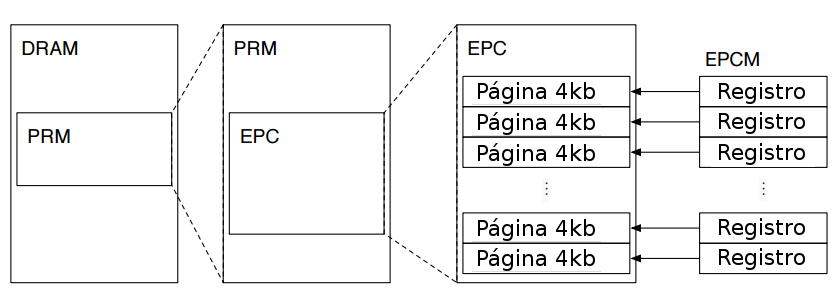
\includegraphics[width=5in]{img/hierarquia_memoria_sgx_pt_BR}
\caption{Hierarquia de memória do Intel SGX}
\label{fig:hierarquiamemoria}
\end{figure}

Intel SGX utiliza uma hierarquia de memória conforme ilustrada na Figura
\ref{fig:hierarquiamemoria}.

Tendo o Intel SGX disponível no processador e habilitado, o BIOS reserva uma
parte da memória principal (DRAM), chamada de \textit{Processor Reserved Memory}
(PRM), e a partir de então o acesso a essa área de memória passa a ser
controlada pelo processador.

Parte da PRM é destinada a uma área de memória conhecida como \textit{Enclave
Page Cache} (EPC). A EPC serve para armazenar páginas de enclaves SGX.
Cada uma dessas páginas é associada a um único enclave SGX. O processador é
responsável por garantir que essas páginas só sejam acessíveis pelo enclave
associado a elas.

Por fim, para auxiliar o controle de acesso à memória, uma estrutura adicional
precisa ser criada. Essa estrutura é conhecida como \textit{Enclave Page Cache
Map} (EPCM), e é utilizada para armazenar metadados -- permissões de leitura,
escrita e execução, tipo, endereço linear, estado, etc. -- sobre as páginas que
residem na EPC.

\subsection{Paginação da EPC}
\label{subsec:sgx_modelo_memoria_paginacao_epc}
De modo a aumentar o número de aplicações protegidas que podem ser suportadas de
forma concorrente, a arquitetura SGX oferece instruções que permitem que
sistemas operacionais façam paginação da EPC de forma segura. O processo de
paginação da EPC também pode ser acionado caso o tamanho dos dados carregados em
um enclave exceda o limite do tamanho da EPC.

O processo de paginação da EPC, em geral, é muito mais custoso que um processo
de paginação normal de um sistema operacional. Isso se deve ao fato de que as
seguintes medidas de segurança devem ser tomadas pelo SGX:

\begin{enumerate}
    \item Uma página de enclave só pode ser removida da EPC depois que todas as
    traduções em cache para essa página tenham sido removidas de todos os
    processadores lógicos;

    \item O conteúdo da página do enclave precisa ser cifrado antes de ser
    escrito na memória principal;

    \item Ao recarregar a página na EPC, informações sobre o tipo, permissões,
    endereço virtual, conteúdo, e o enclave dono da página devem ser
    verificadas, de modo a garantir que as mesmas correspondem à página que foi
    removida;

    \item Apenas a última versão da página removida pode ser recarregada.
\end{enumerate}

\section{Modelo de programação}
\label{sec:sgx_modelo_programacao}

Antes de desenvolver aplicações que fazem uso de Intel SGX, desenvolvedores
devem ter em mente que nem toda a área de sua aplicação deve ser protegida. Na
verdade, a Intel sugere que o mínimo possível da aplicação seja executada dentro
de enclaves SGX -- apenas a parte da aplicação que lida com dados sigilosos.

Dessa forma, aplicações SGX devem ser separadas em duas partes:

\begin{description}
    \item [Parte segura/confiável] -- executada dentro de enclaves SGX. Deve ser
    usada para armazenamento e processamento de dados sensíveis/sigilosos.
    Por ser protegida, há um custo adicional de processamento em comparação com
    a execução de uma aplicação normal, relativo ao processo de cifrar e
    decifrar páginas dos enclaves. Código sendo executado na parte segura não é
    capaz de executar chamadas de sistema.

    \item [Parte insegura/não confiável] -- executada na memória principal da
    máquina. Serve como um invólucro para a parte segura da aplicação, podendo
    ser usado tanto para o processamento de dados que não sejam sigilosos,
    quanto como uma interface de comunicação com outras aplicações ou escrita de
    arquivos.
\end{description}

Para definir como as duas partes da aplicação SGX se comunicam entre si, um
arquivo no formato EDL -- \textit{Enclave Description Language} -- deve ser
provido pelo desenvolvedor. Neste arquivo são definidas funções onde a parte
insegura da aplicação envia dados e executa algum processamento dentro da parte
segura (ECALLs), e funções onde a parte segura da aplicação envia dados e
executa algum processamento na parte insegura (OCalls).

Juntamente com o \textit{SGX SDK} é fornecida uma ferramenta conhecida como
Edger8r. Ela é responsável por ler arquivos EDL e gerar interfaces de
comunicação entre as partes segura e insegura de uma aplicação SGX.

\section{Funcionalidades importantes}
\label{sec:sgx_funcionalidades}

Intel SGX possui algumas funcionalidades que auxiliam no processo de estabelecer
confiança em uma aplicação, bem como no compartilhamento seguro de dados
sigilosos entre diferentes aplicações, ou entre diferentes versões de uma mesma
aplicação. Essas funcionalidades são discutidas a seguir.

\subsection{Medição de enclaves}
\label{subsec:sgx_funcionalidades_medicao_enclaves}

A arquitetura Intel SGX é responsável por estabelecer identidades de enclaves.
No jargão do Intel SGX, o processo de estabelecimento de identidade de um
enclave é conhecido como \textbf{medição de enclave}.
Associadas a cada enclave estão duas identidades distintas:

\begin{description}
    \item [MRENCLAVE] -- Também referido como identidade de enclave, é o
    resultado da função de \textit{hash} SHA-256 do registro de toda a atividade feita ao construir um
    enclave SGX. Em outras palavras, essa identidade é calculada baseada em todo
    o conteúdo carregado em um enclave, \textit{i.e.}, conteúdos das páginas do
    enclave, posição relativa das páginas no enclave, e \textit{flags} de
    segurança associadas às páginas.

    \item [MRSIGNER] -- Também referido como identidade de selagem, é a
    identidade de quem assinou o enclave SGX, tipicamente o desenvolvedor do
    enclave. Múltiplos enclaves podem ser assinados por um mesmo desenvolvedor,
    fazendo com que todos tenham a mesma identidade de selagem.

\end{description}

\subsection{Atestação de enclaves}
\label{subsec:sgx_funcionalidades_atestacao_enclaves}

Atestação é o processo de provar que um determinado programa foi devidamente
instanciado em uma plataforma. No caso do Intel SGX, o processo de atestação
garante que um programa está sendo executado dentro de um enclave SGX, e que não
foram feitas modificações no código do mesmo. O processo de atestação pode ser
feito local ou remotamente.

\subsubsection{Atestação local}
\label{subsubsec:sgx_funcionalidades_atestacao_enclaves_local}

\begin{figure}[ht]
\centering
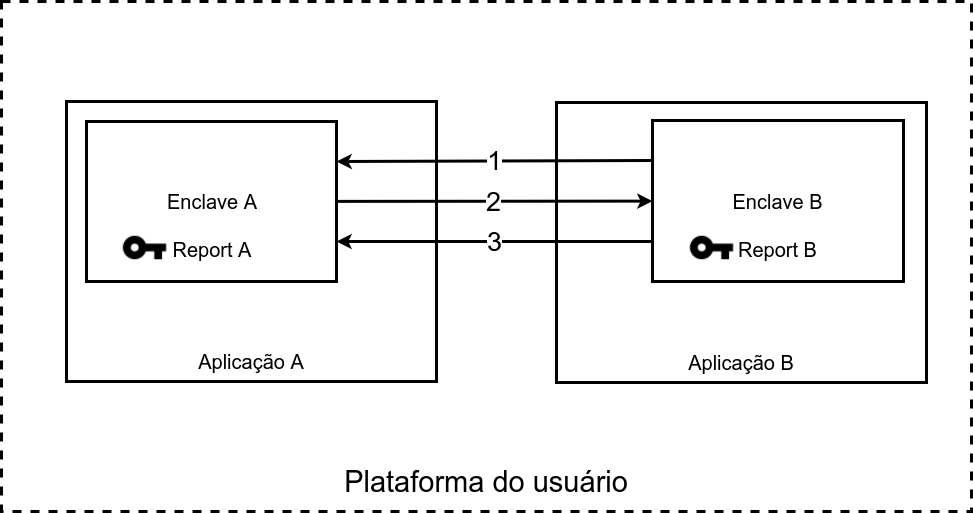
\includegraphics[width=5in]{img/atestacao_local_pt_BR}
\caption{Atestação local}
\label{fig:atestacaolocal}
\end{figure}

Desenvolvedores podem escrever duas ou mais aplicações seguras, executadas em
enclaves, que podem cooperar entre si, para realizar funções que não sejam de
suas próprias competências. Para isso, é provido um mecanismo que permite que
enclaves se autentiquem entre si, através do uso das instruções EREPORT e
EGETKEY.

O processo completo de atestação local de enclaves, ilustrado na Figura
\ref{fig:atestacaolocal}, acontece da seguinte forma:

\begin{enumerate}
    \item Após um canal de comunicação ser estabelecido entre os enclaves A e
    B\footnote{\label{notacomunicacao}Toda comunicação de aplicações SGX passa
    pela parte insegura da aplicação.}, o enclave A obtém o MRENCLAVE do enclave
    B.

    \item O enclave A executa a instrução EREPORT, usando como parâmetro o
    MRENCLAVE do enclave B, criando assim uma estrutura, conhecida como
    \textit{REPORT}, contendo o seu próprio MRENCLAVE e MRSIGNER, e assinada com
    uma chave, \textit{Report Key}, acessível diretamente apenas pelo enclave B.
    Após obtido, o \textit{REPORT} é enviado pelo enclave A para o enclave B.

    \item Tendo recebido o \textit{REPORT} do enclave A:

    \begin{enumerate}
        \item O enclave B executa a instrução EGETKEY para obter a sua chave, e
        com ela, verifica a assinatura do \textit{REPORT} recebido do enclave A.
        Caso a assinatura seja verificada com sucesso, o enclave B pode ter
        certeza que o enclave A está sendo executado na mesma plataforma, que
        por sua vez, está de acordo com o modelo de segurança SGX.

        \item O enclave B pode então verificar se o MRENCLAVE do enclave A,
        contido no \textit{REPORT} recebido, corresponde ao da aplicação com a
        qual ele deseja se comunicar. Em caso positivo, o enclave A pode agora
        ter certeza de estar se comunicando com a aplicação correta.
    \end{enumerate}

\end{enumerate}

O mesmo processo pode ser repetido para que o enclave A confie no enclave B.

\subsubsection{Atestação remota}
\label{subsubsec:sgx_funcionalidades_atestacao_enclaves_remota}

\begin{figure}[ht]
\centering
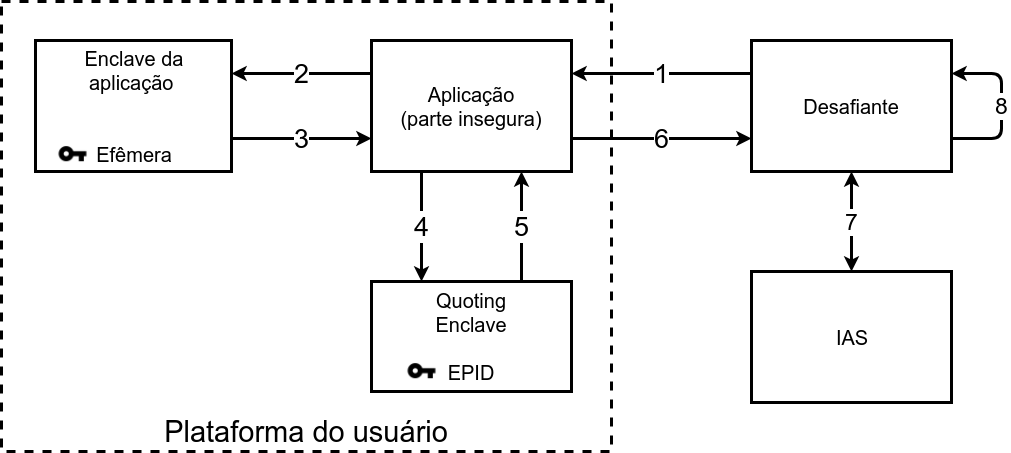
\includegraphics[width=5in]{img/atestacao_remota_pt_BR}
\caption{Atestação remota}
\label{fig:atestacaoremota}
\end{figure}

O processo de atestação local usa um sistema de chaves simétricas, onde a chave
só é acessível através da execução das instruções \textit{EREPORT} e \textit{
EGETKEY}. No caso de uma atestação remota (RA, do inglês \textit{Remote
Attestation}), a aplicação que deseja ganhar confiança em uma aplicação SGX não
é capaz de executar a instrução \textit{EGETKEY}, uma vez que as partes são
executadas em plataformas distintas. Para o processo de atestação remota, é
necessário o uso de um sistema de chaves assimétricas.

Para permitir tal processo, um enclave especial, conhecido como \textit{Quoting
Enclave} (QE), é provido pela Intel. O QE é responsável por usar o processo de
atestação local, e transformar o \textit{REPORT} gerado no processo em uma outra
estrutura, conhecida como \textit{QUOTE}, assinada com uma chave assimétrica,
acessível apenas pelo QE.
Além disso, a Intel provê um serviço de atestação (IAS), que é capaz de
verificar a autenticidade da assinatura de um \textit{QUOTE}.

O processo completo de atestação remota, mostrado na Figura
\ref{fig:atestacaoremota}, acontece da seguinte forma:

\begin{enumerate}
    \item Após estabelecida uma comunicação entre um desafiante e a plataforma
    onde se encontra a aplicação SGX\footref{notacomunicacao}, o desafiante pede
    uma prova de que a aplicação está sendo devidamente executada dentro de um
    enclave SGX. Junto a esse pedido, o desafiante envia a sua chave pública.

    \item Recebendo tal pedido, o enclave procede criando uma estrutura,
    \textit{MSG1}, que contém sua chave pública, e a envia para o desafiante.

    \item Em seguida, o desafiante é capaz de derivar uma chave
    simétrica, \textit{SMK}, através do método \textit{Diffie-Hellman}, usando a
    sua chave privada e a chave pública do enclave. Tendo essa chave simétrica
    em mãos, o desafiante deve gerar uma outra estrutura, \textit{MSG2}, e
    enviar para o enclave. A \textit{MSG2} contém:
    \begin{enumerate}
        \item a chave pública do desafiante;
        \item um identificador de registro do desafiante para com o IAS;
        \item uma assinatura da concatenação de ambas as chaves públicas, usando
        a chave privada do desafiante;
        \item um código de autenticação de mensagem (MAC) de toda a mensagem,
        usando a chave \textit{SMK}, que pode ser verificada pelo enclave.
    \end{enumerate}

    \item O enclave deve então gerar o seu \textit{REPORT}, e enviar para o QE,
    para que ele gere o \textit{QUOTE} do enclave.

    \item O enclave gera um \textit{MAC} do \textit{QUOTE} recebido, usando a
    chave \textit{SMK}, e a envia para o desafiante.

    \item O desafiante verifica o \textit{MAC}, para garantir que está se
    comunicando com o mesmo enclave ainda, e após verificar com sucesso, envia o
    \textit{QUOTE} para o \textit{IAS}.

    \item O \textit{IAS} verifica se a assinatura e a estrutura do \textit{QUOTE}
    são válidos, ou seja, foram gerados por um enclave SGX, e envia um resposta
    para o desafiante.

    \item Tendo confirmado a validade do \textit{QUOTE}, o desafiante verifica
    se o \textit{MRENCLAVE}, contido no \textit{QUOTE}, é o esperado,
    completando assim o processo de atestação remota.

\end{enumerate}

Após completar o processo de atestação remota, ambas as partes envolvidas podem
usar a chave \textit{SMK} para enviar mensagens entre si de forma segura.

\subsection{Selagem de dados}
\label{subsec:sgx_funcionalidades_selagem_dados}

Enquanto um enclave está instanciado, o \textit{hardware} garante a integridade
e confidencialidade de seus dados. Entretanto, ao encerrar o processo de um
enclave, todo o seu conteúdo é destruído, e qualquer dado que esteja no enclave
será perdido.

Se os dados do enclave seriam usados posteriormente, \textit{e.g.}, em uma
futura execução do enclave, é necessário que esses dados sejam armazenados fora
da área protegida do enclave.
Com este objetivo, o SGX provê uma funcionalidade para selar estes dados e
armazená-los em disco de forma segura.
A funcionalidade de selagem de dados pode ser feita de duas formas:

\begin{description}
    \item [Selagem usando a Identidade de enclave] -- Utilizada quando apenas o
    mesmo código de enclave deve ser capaz de acessar os dados selados. Utiliza
    o MRENCLAVE para selar os dados.
    Com essa forma de selagem, não é possível transferir dados para aplicações
    diferentes, ou até mesmo para uma nova versão da mesma aplicação.

    \item [Selagem usando a Identidade de selagem] -- Utilizada quando se deseja
    transferir dados de um enclave para uma aplicação distinta ou para uma nova
    versão da mesma aplicação. Utiliza o MRSIGNER para selar os dados.
    Os dados selados serão acessíveis por qualquer enclave que tenha sido
    assinado pelo mesmo desenvolvedor, o que resulta em um mesmo MRENCLAVE.
    Também é útil quando se deseja atualizar uma aplicação, \textit{e.g.},
    quando deseja-se usar um código mais eficiente ou mais seguro na aplicação.
\end{description}

\section{Ciclo de vida de aplicações SGX}
\label{sec:sgx_ciclo_vida}

\begin{figure}[ht]
\centering
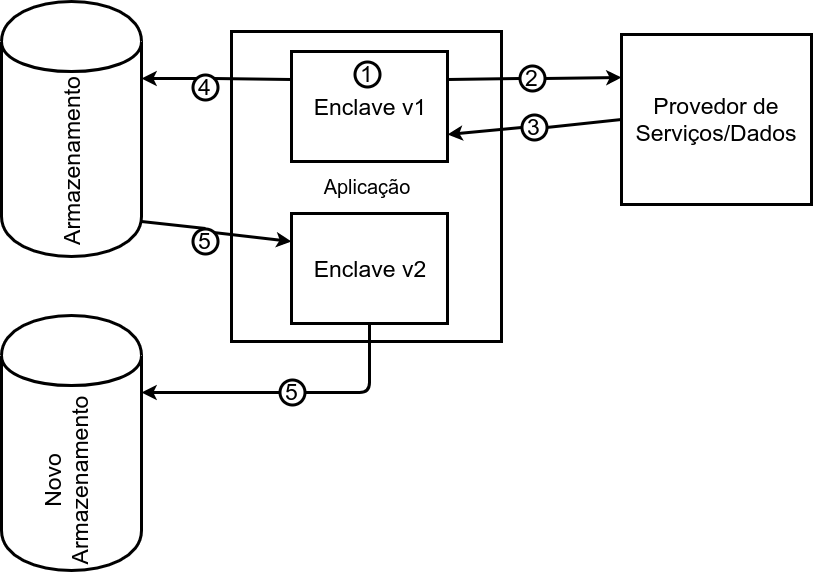
\includegraphics[width=5in]{img/ciclovida_sgx}
\caption{Ciclo de vida de aplicações SGX}
\label{fig:ciclovida}
\end{figure}

Aplicações SGX devem ser iniciadas sem conter nenhum dado sigiloso na memória.
Depois que o enclave SGX já está sendo executado, o processo de atestação de
enclaves pode ser usado para obter confiança em uma aplicação SGX, e estabelecer
um canal de comunicação seguro, para enviar dados para serem processados dentro
do enclave da aplicação SGX.

A aplicação SGX pode cifrar os seus dados e armazená-los para um uso futuro,
usando a funcionalidade de selagem de dados.

A Figura \ref{fig:ciclovida} ilustra os passos dados para completar esse ciclo.

\begin{enumerate}
    \item Inicialização de enclave -- A parte insegura da aplicação é
    responsável por criar o enclave. No processo de inicialização do enclave o
    seu MRENCLAVE é calculado.

    \item Atestação -- A aplicação SGX usa o processo de atestação remota para
    se tornar confiável e estabelecer um canal de comunicação seguro.

    \item Provisionamento -- A aplicação SGX recebe os dados sigilosos através
    do canal de comunicação seguro.

    \item Selagem -- O enclave usa a funcionalidade de selagem para armazenar
    seus dados sigilosos de forma que uma nova versão da aplicação possa
    acessá-los.

    \item Atualização de aplicação -- Uma aplicação SGX pode necessitar de uma
    atualização, e sua versão atualizada recebe os dados da versão anterior.

\end{enumerate}

\section{Intel SGX SDK e PSW}
\label{sec:sgx_sdk_psw}

O SDK é um conjunto de ferramentas e APIs com funções de alto nível (em C/C++)
que permite a criação e uso de enclaves SGX de forma mais fácil para o
desenvolvedor.
Juntamente com o SDK estão presentes duas ferramentas essenciais no ciclo de
vida de aplicações SGX. São elas:

\begin{itemize}
    \item sgx\_edger8r -- responsável por criar as interfaces de comunicação
    entre as partes segura e insegura da aplicação.

    \item sgx\_sign -- responsável por assinar um enclave SGX, usando uma chave
    privada, que resultará no MRSIGNER do enclave.
\end{itemize}

Já o PSW, distribuído junto do SDK, trata-se de um conjunto de enclaves especias
da Intel, usados para instanciar e realizar o processo de medição enclaves.
Entre os enclaves mais importantes estão:

\begin{itemize}
    \item \textit{Launch Enclave} (LE) -- responsável por instanciar enclaves
    SGX.

    \item \textit{Quoting Enclave} (QE) -- responsável por gerar a estrutura
    conhecida como QUOTE, usada no processo de atestação remota de enclaves SGX.

    \item \textit{Provisioning enclave} (PvE) -- responsável por prover chaves
    necessárias ao processo de atestação de um enclave.
\end{itemize}

Ambos o SDK e o PSW estão disponíveis tanto para a plataforma \textit{Windows}
quanto para a plataforma \textit{Linux}\footnote{\label{fn:SGXSDK}\url
{https://software.intel.com/en-us/sgx-sdk/download}}.

\section{Casos de uso de SGX}
\label{sec:sgx_casos_de_uso}

Considerando aplicações do tipo cliente-servidor que usam SGX, podemos observar
dois modelos: ($i$) proteção de dados no lado do cliente, ou ($ii$) proteção de
dados no lado do servidor.

\subsection*{Máquina cliente como \textit{host} do enclave SGX}

Neste modelo de aplicação, o objetivo é ter uma aplicação na máquina cliente que
\textbf{obtém} dados sensíveis de algum provedor de serviços. Antes de receber
tais dados, a aplicação precisa provar para o provedor de serviços que está
sendo executada em um enclave SGX.

Como exemplo de aplicação que pode tirar proveito de SGX para proteção de dados
sigilosos, podemos citar uma aplicação de \textit{Internet Banking}. Neste caso,
a entidade financeira em posse dos dados de um cliente precisa se certificar que
os dados sensíveis, \textit{e.g.}, saldo e extrato de conta, só serão acessíveis
pelo cliente a quem a conta pertence. Para alcançar este objetivo, a entidade
financeira pode desenvolver uma aplicação que execute dentro de um enclave SGX,
e que seja atestável pelo seu provedor de serviços.

Outro caso de uso deste modelo que podemos citar é o de gestão de direitos
digitais (DRM, do inglês \textit{Digital Rights Management}). Neste caso, um
enclave SGX pode ser utilizado para evitar que cópias de conteúdos digitais
sejam feitas sem a devida autorização. Uma grande empresa que atualmente está
utilizando Intel SGX para este fim é a Netflix\footnote{\url
{https://help.netflix.com/pt/node/55763}}. Ela utiliza as capacidades do SGX
para proteger vídeos transmitidos com qualidade 4K.

\subsection*{Máquina servidora como \textit{host} do enclave SGX}

Neste modelo de aplicação, o objetivo é ter uma aplicação na máquina cliente que
\textbf{envia} dados sensíveis para algum provedor de serviços. Antes de enviar
tais dados, a aplicação precisa ter certeza que está se comunicando com um
provedor de dados confiável, \textit{i.e.}, está executando em um enclave SGX.

Um caso de uso que podemos citar como exemplo deste modelo é o de agregação de
dados de \textit{smart meters}~\cite{sac2017}. Neste caso, \textit{smart meters}
coletam dados de consumo de energia de residências com um alto nível de detalhe.
Estes dados podem ser usados para derivar informações sobre os indivíduos que
ali residem\footnote{\url{https://www.cnet.com/news/researchers-find-smart-
meters-could-reveal-favorite-tv-shows/}}. Desta forma, é necessário prover um
certo nível de proteção destes dados, para que eles só possam ser utilizados
de forma agregada por distribuidores de energia.

\section{Limitações do Intel SGX}
\label{sec:sgx_limitacoes}

Como qualquer outra tecnologia, Intel SGX também possui limitações. As mais
importantes delas são discutidas a seguir.

\subsection{Privacidade de código}
\label{subsec:sgx_limitacoes_privacidade_codigo}

Apesar de dar garantias quanto à proteção do código de aplicações contra
modificações não autorizadas, Intel SGX não garante a privacidade desse mesmo
código. Em outras palavras, arquivos contendo todo o código de um enclave SGX
são carregados na memória principal de forma não cifrada.

Há vários cenários onde desenvolvedores desejam manter a privacidade de seu
código, portanto essa limitação deve ser levada em consideração por
desenvolvedores, uma vez que atacantes poderiam facilmente usar ferramentas como
o IDA \cite{idapro} para gerar um pseudo-código bastante similar à aplicação
original.

\subsection{Ligação estática de bibliotecas}
\label{subsec:sgx_limitacoes_ligacao_estatica}

Aplicações que usam bibliotecas de terceiros precisam ligar tais bibliotecas a
seus enclaves estaticamente. Isso pode resultar em um enclave demasiadamente
grande, e, consequentemente desperdiçar espaço da memória, que é um recurso
bastante escaço para o SGX. Outra consequência desta limitação é que qualquer
mínima modificação em uma única biblioteca pela aplicação requer que toda a
aplicação SGX seja completamente recompilada e reimplantada.

\subsection{Memória disponível}
\label{subsec:sgx_limitacoes_memoria}

O espaço da memória principal usado pela PRM deve ser reservado pelo BIOS no
momento em que o sistema está sendo inicializado. Além disso, toda a EPC deve
residir dentro da PRM. Na versão atual do SGX, a parte da memória reservada para
a PRM é limitada a um tamanho máximo de apenas $128\ MB$ por máquina. Caso o espaço
necessário seja maior do que o disponível, há um grande aumento no tempo de
processamento, devido ao custoso processo de paginação entre EPC e DRAM,
conforme descrito na seção~\ref{subsec:sgx_modelo_memoria_paginacao_epc}. Na
seção~\ref{sec:abordagem_gerencia_memoria} discutiremos melhor os impactos da
gerência de memória protegida.

\subsection{Vulnerabilidades}
\label{subsec:sgx_limitacoes_vulnerabilidades}

Conforme descrito na Seção~\ref{sec:sgx_modelo_ameaca}, aplicações SGX podem ser
vulneráveis a ataques de canal lateral. Esse tipo de ataque permite que um
adversário colete estatísticas sobre execução da \textbf{CPU}, e as utilize para
deduzir características sobre o programa em execução. Apesar de SGX não prover
proteção contra esse tipo de ataque, é possível previní-lo, tomando os devidos
cuidados\footnote{\url
{https://github.com/chowes/sgx-side-channel/blob/master/sgx-side-channel.pdf}}.

É importante notarmos também que a solução de SGX é composta por componentes --
\textit{drivers}, bibliotecas, e instruções -- complexos, e, portanto,
dificilmente é completamente livre de erros, como qualquer outro
\textit{software}. Além disso, desenvolvedores de aplicações SGX podem cometer
erros e escrever enclaves suscetíveis a vulnerabilidades como \textit
{buffer overflow} e formatação não verificada de \textit{strings}.

Uma técnica de segurança que tem suas funcionalidades limitadas com o uso de SGX
é a de aleatorização do leiaute do espaço de endereçamento (ASLR, do inglês
\textit{Address Space Layout Randomization}). Esta técnica torna aleatória a
organização na memória de diversas partes de um processo, evitando assim que
atacantes usem as vulnerabilidades mencionadas anteriormente para desviar a
execução de um programa para uma função explorada carregada na memória. No
caso do SGX, por ter um espaço de endereçamento reduzido, ataques de força bruta
podem ser utilizados para descobrir o endereço desejado. Em experimentos
realizados, foi verificado que em diferentes execuções, uma variável de um
enclave SGX tem seu endereço modificado em apenas dois \textit{bytes},
significando que a aleatorização tem aproximadamente apenas $65536$
possibilidades. Essa quantidade de possibilidades é muito pequena, uma vez que
atacantes podem aumentar a probabilidade de ataques com sucesso através da
injeção de sequências de instruções \textbf{NOP} antes de um código malicioso.

\section{Considerações}

Intel SGX é uma tecnologia bastante promissora, oferecendo garantias de
segurança e privacidade de dados de usuários contra ataques provenientes até
mesmo de atacantes que tenham obtido privilégio indevidamente, ou que tenham
acesso físico à máquina que hospeda os dados sigilosos. Como qualquer outra
tecnologia, porém, também possui limitações que podem pôr em risco a sua
aplicabilidade no mundo real. É necessário, portanto, fazer uma análise dos
principais desafios a serem enfrentados durante o processo de desenvolvimento de
aplicações que façam uso desta tecnologia, antes de pô-la em um ambiente de
produção.
\chapter{Características-chaves em aplicações SGX}
\label{chapter:abordagem}

Neste capítulo, detalhamos a abordagem utilizada neste trabalho, que envolve a
avaliação do impacto de características de aplicações SGX na performance e na
segurança providas pelas mesmas. Para cada uma das características avaliadas
neste trabalho, realizamos vários experimentos. Para os experimentos dispomos de
uma máquina Dell Optiplex 5040, com um processador Intel Core i7-7700, com 4
núcleos operando a $3,4\ GHz$, e $8\ GB$ de memória principal disponível.

De forma a mensurar o impacto de cada uma das características, coletamos e
analisamos duas métricas: ($i$) o tamanho do TCB gerado -- lembrando que quanto
maior o TCB, maior a probabilidade de se inserir \textit{bugs} e
vulnerabilidades no mesmo -- impactando diretamente a segurança de uma
aplicação, e ($ii$) tempo de processamento das aplicações.

Em cada uma das seções a seguir, apresentamos as principais características que
devem ser consideradas durante o desenvolvimento de aplicações SGX, incluindo
uma descrição dos experimentos realizados, resultados obtidos nos experimentos,
e uma discussão sobre os impactos de tais características nas aplicações em
questão.  

\section{Gerência de memória}
\label{sec:abordagem_gerencia_memoria}

Conforme apontado na Seção~\ref{sec:sgx_limitacoes}, uma das limitações de SGX é
a pequena área de memória protegida pela tecnologia, com apenas $128\ MB$
disponíveis.
Nesta seção, avaliamos os possíveis impactos na performance de aplicações SGX,
caso elas venham a ter um consumo de memória que exceda o limite de memória
disponível.

\begin{lstlisting}[language=C, label=lst:acesso_aleatorio, caption={Pseudocódigo
do experimento de acesso aleatório à memória.}]
    #define MB_SIZE 1024*1024

    char tmp;

    char perform_random_memory_access(int size_in_mb) {
        size_t total_size = size_in_mb * MB_SIZE;
        char *allocated_memory = (char *) malloc(total_size);
        
        int i;
        for (i=0; i<total_size; ++i) {
            int pos = rand() % total_size; // A função rand() gera um número aleatório.
            tmp ^= allocated_memory[pos]; // Para evitar otimizações feitas pelo compilador.
        }
        free(allocated_memory);
        return tmp;
    }
\end{lstlisting}

\subsection*{Experimentos}

Para avaliar o impacto do consumo de memória em aplicações SGX, realizamos um
experimento que compara o desempenho de acesso aleatório à memória em uma
aplicação escrita em C, sem garantias de segurança, e em uma aplicação que usa
SGX, com garantias de segurança. As implementações de ambas aplicações são
praticamente idênticas, diferindo apenas que a alocação e acesso aleatório de
memória da aplicação SGX são feitos dentro de um enclave, enquanto na primeira
implementação são feitos de forma insegura.

O código utilizado em ambas implementações é exibido no Código Fonte~\ref
{lst:acesso_aleatorio}, e é descrito da seguinte forma:

\begin{enumerate}
    \item A aplicação aloca um espaço de memória do tamanho passado como
    parâmetro, associando-o à variável \textit{allocated\_memory}, que será
    utilizada como um \textit{array} de elementos do tipo \textit{char}
    (linha 7);
    \item A aplicação gera um número inteiro aleatório $pos$, que indica o
    índice do \textit{array} a ser acessado (linha 11);
    \item A aplicação acessa o elemento presente no índice aleatório gerado
    (linha 12);
    \item A aplicação repete os passos 2 e 3 pelo número de vezes que
    corresponde ao total de posições do \textit{array} alocado (linhas 10-13);
    \item A aplicação libera o espaço alocado para a variável \textit
    {allocated\_memory} (linha 14).
\end{enumerate}

Neste experimento o espaço de memória utilizado pelas aplicações foi variado
entre $1\ MB$ e $1024\ MB$, em uma escala logarítmica.

Tendo em vista que, neste experimento, apenas o tamanho da memória alocada e
acessada aleatoriamente é variada, coletamos apenas a métrica do tempo de
processamento tanto para a aplicação insegura, em C puro, e a aplicação segura,
utilizando SGX.

\subsection*{Resultados obtidos}

\begin{figure*}[!t]
    \centering
    \subfloat[Tamanho de memória variando entre 1MB e 1024MB]
    {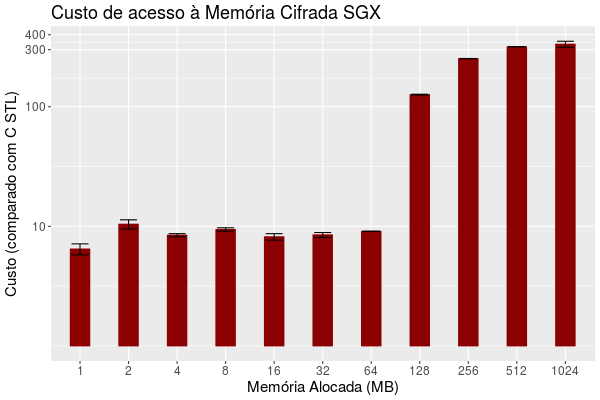
\includegraphics[width=5in]{img/memory-benchmark-1-1024-br}
    \label{fig:sgx_memory_overhead_1024}}
    \hfil
    \subfloat[Tamanho de memória variando entre 64MB e 128MB]
    {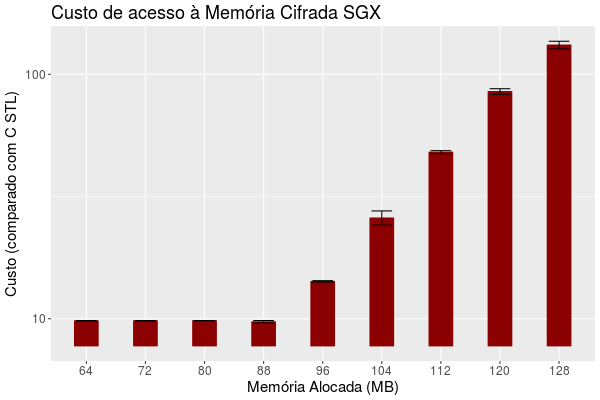
\includegraphics[width=5in]{img/memory-benchmark-64-128-br}
    \label{fig:sgx_memory_overhead_64}}
    \caption{Sobrecarga média de acesso à memória SGX comparado com acesso à
    memória em C puro, com um intervalo de 95\% de confiança.}
    \label{fig:sgx_memory_overhead}
\end{figure*}

Para cada uma das configurações descritas anteriormente, trinta repetições do
experimento foram executadas.
A Figura \ref{fig:sgx_memory_overhead} mostra a relação entre os tempos de
execução da aplicação SGX e da aplicação C pura, considerando cada uma das
configurações determinadas anteriormente. Na Figura~\ref
{fig:sgx_memory_overhead_1024}, notamos que aplicações SGX que usam até $64\ MB$ de
memória têm um custo médio de acesso à memória aproximadamente $10$ vezes mais
alto que aplicações sem garantias de segurança. Já aplicações que consumam $128\ MB$
de memória ou mais têm um custo médio de acesso à memória pelo menos $100$ vezes,
e chegando a ser $380$ vezes mais alto que o de aplicações inseguras.

Para entender melhor o comportamento do custo de acesso à memória em aplicações
SGX, repetimos o experimento descrito anteriormente, porém variando o espaço de
memória utilizado entre $64\ MB$ e $128\ MB$, com incrementos de $8\ MB$. Na Figura~\ref
{fig:sgx_memory_overhead_64}, podemos observar que aplicações que demandam até
88MB de memória têm um custo médio de acesso à memória $10$ vezes mais alto que
aplicações inseguras. Aplicações que ultrapassem $88\ MB$ têm um custo de acesso que
cresce linearmente à medida que mais memória é demandada.

\subsection*{Discussão}

Considerando os resultados obtidos nestes experimentos, podemos concluir que a
quantidade de memória consumida e uma gerência de memória apropriada são
características de extrema importância no desenvolvimento de aplicações SGX,
visto que um alto consumo de memória pode torná-las impraticáveis no mundo real.
Dados os resultados obtidos nos experimentos aqui apresentamos, recomendamos que
desenvolvedores busquem criar e utilizar suas aplicações de um modo que ela não
consuma além do limite de memória disponível na EPC, sob o risco de obter uma
sobrecarga demasiadamente alta no tempo de processamento de sua aplicação, caso
essa recomendação não seja seguida.

É importante notar que, apesar de termos reservado um espaço de $128\ MB$ para a
PRM, apenas cerca de $90\ MB$ ficam disponíveis para a EPC. Isso de deve ao fato de
que parte da PRM é utilizada pela estrutura EPCM e pelos enclaves especiais da
Intel.

\section{Particionamento de dados}
\label{sec:abordagem_particionamento_dados}

Existem aplicações que precisam processar um grande volume de dados, também
conhecido como processamento de \textit{Big Data}. Considerando esse tipo de
aplicações, desejamos analisar qual a melhor forma para processar este grande
volume de dados, desde que sejam independentes entre si. Nesta seção,
procura-se, mais precisamente, saber se, e como, este grande volume de dados
independentes deve ser particionado para ser processado dentro de enclaves SGX,
considerando-se a disponibilidade de um único enclave. Em outras palavras,
deseja-se identificar como particionar um grande volume de dados para processar
suas partes independentes, sequencialmente, da forma mais eficiente possível.

\subsection*{Experimentos}

A característica que avaliamos nesta seção envolve apenas variações na carga
útil a ser processada, e não na aplicação SGX usada para processar estes dados.
Desta forma, o tamanho do TCB não será uma métrica coletada e avaliada nestes
experimentos, uma vez que o tamanho do TCB permanece constante em todas as
configurações. A métrica coletada e avaliada nesta seção é o tempo de execução
necessário para completar a tarefa de computar a soma de todos os elementos de
um \textit{array} de números inteiros com 1GB de tamanho.

Este experimento, foi dividido em duas partes. Em um primeiro momento, buscou-se
avaliar o tempo de processamento do \textit{array}, considerando-se partições
com tamanhos de $1$, $2$, $4$, $8$, $16$, $32$, $64$, $128$, $256$, $512$, e
$1024\ MB$. Em um segundo momento, tendo em vista as observações de perda de
desempenho quando enclaves excedem o tamanho disponível na EPC, feitas na
Seção~\ref{sec:abordagem_gerencia_memoria}, buscou-se avaliar também o tempo de
processamento do \textit{array}, considerando-se partições com tamanhos de $72$,
$80$, $88$, $96$, $104$, e $112\ MB$.

\begin{lstlisting}[language=C, label=lst:particionamento_dados, caption={Pseudocódigo
do experimento de particionamento de dados.}]
    // Na parte insegura da aplicação

    #define MB_SIZE 1024*1024
    
    long sum_array(int chunk_size_in_mb){
        int array_size = 1024 * MB_SIZE;
        int chunk_size = chunk_size_in_mb * MB_SIZE;
        int *array = generate_random_array(array_size); // Cria um array com tamanho 1GB
        long sum = 0;
        int i;
        for (i=0; i<array_size/chunk_size; ++i){
            sum += enclave_sum(&array[i*chunk_size], chunk_size);
        }
        free(allocated_memory);
        return sum;
    }

    // No enclave da aplicação

    long enclave_sum(int *array, int array_size){
        long sum = 0;
        int i;
        for (i=0; i<array_size; ++i){
            sum += array[i];
        }
        return sum;
    }
\end{lstlisting}

O código utilizado neste experimento é exibido no Código Fonte~\ref
{lst:particionamento_dados}, e é descrito da seguinte forma:

\begin{enumerate}
    \item A aplicação aloca um espaço de memória com tamanho de $1\ GB$,
    associando-o à variável \textit{array}, que é um \textit{array} de elementos
    do tipo \textit{int} (linha 8);
    \item A aplicação envia para o enclave uma partição dos dados para calcular
    a soma dos elementos desta partição (linha 12);
    \item O enclave da aplicação calcula a soma dos elementos da partição
    recebida (linhas 23-25);
    \item Repetimos os passos 2 e 3 até que a soma de todas as partições tenham
    sido computadas (linhas 11-13);
    \item A aplicação libera o espaço alocado para a variável \textit{array}
    (linha 14).
\end{enumerate}

É importante salientar que o tamanho do \textit{array} copiado para o enclave a
cada chamada à função \textit{enclave\_sum} é exatamente o tamanho passado pelo
parâmetro \textit{array\_size} da mesma função. O número de chamadas feitas à
função \textit{enclave\_sum}, considerando cada um dos tamanhos de partição
propostos, pode ser visto na Tabela~\ref
{tab:abordagem_particionamento_dados_chamadas}.

\begin{center}
    \begin{table}
        \caption{Número de chamadas à função \textit{enclave\_sum} necessárias
        para computar a soma dos elementos de um \textit{array} com 1GB de
        tamanho, de acordo com o tamanho, em MB, das partições.}
        \label{tab:abordagem_particionamento_dados_chamadas}
        \centering
        \begin{tabular}{|c|c|c|c|c|}
            \cline{1-2} \cline{4-5}
            \textbf{Tam. da partição} & \textbf{Num. de chamadas} & & \textbf{Tam. da partição} & \textbf{Num. de chamadas} \\
            \cline{1-2} \cline{4-5}
            1 & 1024 & & 88 & 12 \\
            \cline{1-2} \cline{4-5}
            2 & 512 & & 96 & 11 \\
            \cline{1-2} \cline{4-5}
            4 & 256 & & 104 & 10 \\
            \cline{1-2} \cline{4-5}
            8 & 128 & & 112 & 10 \\
            \cline{1-2} \cline{4-5}
            16 & 64 & & 120 & 9 \\
            \cline{1-2} \cline{4-5}
            32 & 32 & & 128 & 8 \\
            \cline{1-2} \cline{4-5}
            64 & 16 & & 256 & 4 \\
            \cline{1-2} \cline{4-5}
            72 & 15 & & 512 & 2 \\
            \cline{1-2} \cline{4-5}
            80 & 13 & & 1024 & 1 \\
            \cline{1-2} \cline{4-5}
        \end{tabular}
    \end{table}
\end{center}

\subsection*{Resultados obtidos}

\begin{figure*}[!t]
   \centering
   \subfloat[Tamanho da partição variando entre 1MB e 1024MB]
   {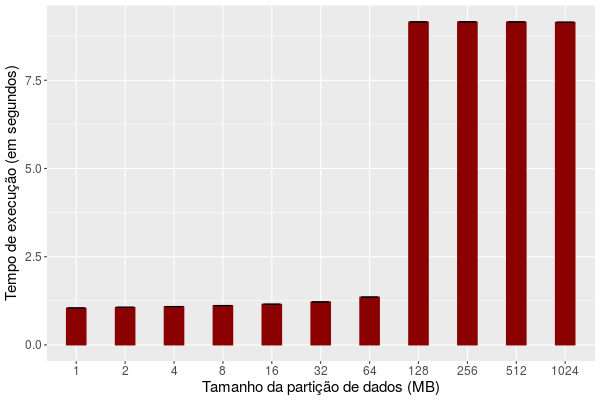
\includegraphics[width=5in]{img/particionamento-dados-1-1024-final}
   \label{fig:abordagem_particionamento_dados_1024}}
   \hfil
   \subfloat[Tamanho da partição variando entre 64MB e 128MB]
   {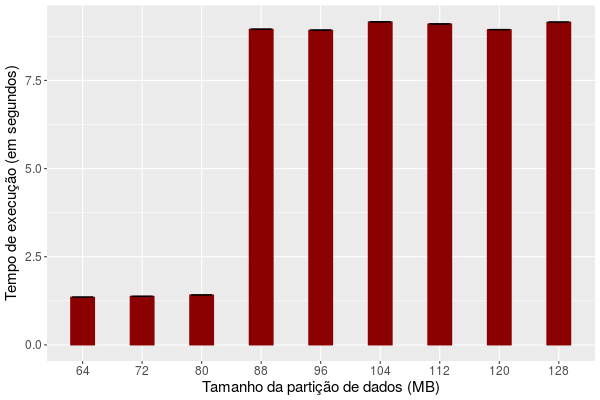
\includegraphics[width=5in]{img/particionamento-dados-64-128-final}
   \label{fig:abordagem_particionamento_dados_128}}
   \caption{Tempos médios para calcular a soma dos elementos de um \textit
   {array} com tamanho de 1GB, variando o tamanho das partições utilizadas
   no cálculo das somas parciais, com um intervalo de 95\% de confiança.}
   \label{fig:abordagem_particionamento_dados}
\end{figure*}

A Figura~\ref{fig:abordagem_particionamento_dados} mostra o tempo total de
processamento do \textit{array} com tamanho de $1\ GB$, em cada um dos cenários
propostos. A partir dos resultados exibidos na Figura~\ref
{fig:abordagem_particionamento_dados_1024}, notamos que, para o particionamento
de dados feito com partições de até $64\ MB$, à medida que o tamanho das partições
cresce, o tempo total de execução da tarefa também cresce -- o tempo de execução
usando partições com tamanho de $64\ MB$ é cerca de $28\%$ mais alto que o tempo de
execução usando partições com tamanho de $1\ MB$. Já para o particionamento de dados
feito com partições de $128\ MB$ ou mais, é notável a sobrecarga gerada pelo consumo
de memória superior ao disponibilizado na EPC, porém não há, estatísticamente,
diferença entre o uso de diferentes tamanhos de partições que excedam este
limite -- o tempo de execução da tarefa usando partições de $1024\ MB$ é cerca de
$0,6\%$ mais baixo que o tempo de execução usando partições de $128\ MB$.

Analisando os dados exibidos na Figura~\ref
{fig:abordagem_particionamento_dados_128}, podemos dizer que a sobrecarga no
tempo de execução da tarefa pode ser observado quando particionamos os dados em
partições com tamanho de $88\ MB$ ou mais, gerando um tempo de execução pelo menos
$534\%$ mais alto que o uso de partições que não extrapolam o limite da EPC.

\subsection*{Discussão}

Mais uma vez, podemos notar que o limite de memória disponível na EPC é um dos
fatores-chave no desenvolvimento de aplicações SGX. Mais especificamente,
mostramos com estes experimentos que é essencial que grandes volumes de dados
sejam particionados antes de serem processados em aplicações SGX. Dados os
resultados obtidos, recomendamos que grandes volumes de dados sejam
particionados em pedaços tão pequenos quanto possível, e evitar a todo custo
processar pedaços de dados que excedam o tamanho de $80\ MB$.

\section{Particionamento de aplicações}
\label{sec:abordagem_particionamento_aplicacoes}

Conforme exposto na Seção~\ref{sec:sgx_modelo_programacao}, aplicações SGX são
divididas entre parte segura, \textit{i.e.}, enclave que protege dados contra
modificação ou acesso não autorizados, e parte insegura, \textit{i.e.}, código
em volta do enclave, que serve para processar dados não-sensíveis, e  para
estabelecer uma comunicação entre o enclave e outras aplicações. Desta forma,
nesta seção, buscamos analisar qual a melhor forma de particionar aplicações
SGX, de modo que sua performance e sua segurança não sejam comprometidas.

\subsection*{Experimentos}

A característica que avaliamos nesta seção envolve variações na divisão de uma
aplicação, com o objetivo de torná-la segura, através do uso de SGX. Deste modo,
coletamos tanto o tempo de execução necessário para completar a tarefa de
computar a soma de um número variado de elementos, como fazemos considerações
sobre o TCB resultante.

Neste experimento, consideramos uma aplicação simples, que tem como funções
($i$) gerar e ($ii$) computar a soma de uma quantidade $N$ de números inteiros.
Para realizar esta tarefa, consideramos duas implementações. A primeira delas,
exibida no Código Fonte~\ref{lst:particionamento_aplicacoes_enclave}, realiza
ambas as funções dentro do enclave, gerando um maior TCB, mas mantendo todo o
processamento dentro do enclave, e é descrita da seguinte forma:

\begin{enumerate}
    \item O enclave inicializa a variável \textit{sum} com o valor $0$ (linha
    10);
    \item O enclave gera um novo número (linhas 3-7 e linha 13);
    \item O enclave soma o novo número à variável \textit{sum} (linha 14);
    \item O enclave repete $N$ vezes os passos 2 e 3, até obter o resultado
    final (linhas 12-15).
\end{enumerate}


A segunda implementação, exibida no Código Fonte~\ref
{lst:particionamento_aplicacoes_mista}, por sua vez, realiza a função de somar
os elementos dentro do enclave, enquanto a função de gerar o próximo elemento é
realizada pela parte insegura da aplicação, gerando um TCB reduzido, mas
executando um grande número interações entre as partes segura e insegura através
de OCalls. Esta implementação é descrita da seguinte forma:

\begin{enumerate}
    \item O enclave inicializa a variável \textit{sum} com o valor $0$ (linha
    10);
    \item O enclave solicita um novo número através da chamada da OCall \textit
    {ocall\_generate\_number} (linha 14);
    \item A parte insegura gera um novo número (linhas 3-6);
    \item O enclave soma o novo número à variável \textit{sum} (linha 15);
    \item Repetimos $N$ vezes os passos 2, 3 e 4, até obter o resultado final
    (linhas 13-16).
\end{enumerate}

\begin{lstlisting}[language=C, label=lst:particionamento_aplicacoes_enclave,
    caption={Pseudocódigo do experimento de particionamento de aplicações, com
    todas as tarefas executadas no enclave.}]
    // No enclave da aplicação
    
    int generate_number(){
        int res;
        sgx_read_rand(&res, sizeof(int));
        return res;
    }
        
    long enclave_calculate_sum(int N){
        long sum = 0;
        int i, next_number;
        for (i=0; i<N; ++i){
            next_number = generate_number();
            sum += next_number;
        }
        return sum;
    }
\end{lstlisting}
\begin{lstlisting}[language=C, label=lst:particionamento_aplicacoes_mista,
caption={Pseudocódigo do experimento de particionamento de aplicações, com as
tarefas separadas entre o enclave e a parte insegura.}]
    // No parte insegura da aplicação
    
    int ocall_generate_number(){
        int res = rand() % 100;
        return res;
    }

    // No enclave da aplicação

    long enclave_calculate_sum(int N){
        long sum = 0;
        int i, next_number;
        for (i=0; i<N; ++i){
            ocall_generate_number(&next_number);
            sum += next_number;
        }
        return sum;
    }
\end{lstlisting}

Neste experimento, o número de valores gerados, $N$, em ambas implementações foi
variado entre $100$ e $100000000$, em uma escala logarítmica.

\subsection*{Resultados obtidos}

A Figura~\ref{fig:abordagem_particionamento_aplicacoes} mostra a comparação do
tempo de execução de ambas implementações descritas, considerando cada uma das
confirgurações determinadas. Neste experimento, podemos notar que a
implementação que gera os valores fora do enclave e o soma ao resultado parcial
é, em todos os casos, cerca de $20$ vezes mais lenta que a implementação que
realiza ambas as funções dentro do enclave.

\begin{figure}[ht]
    \centering
    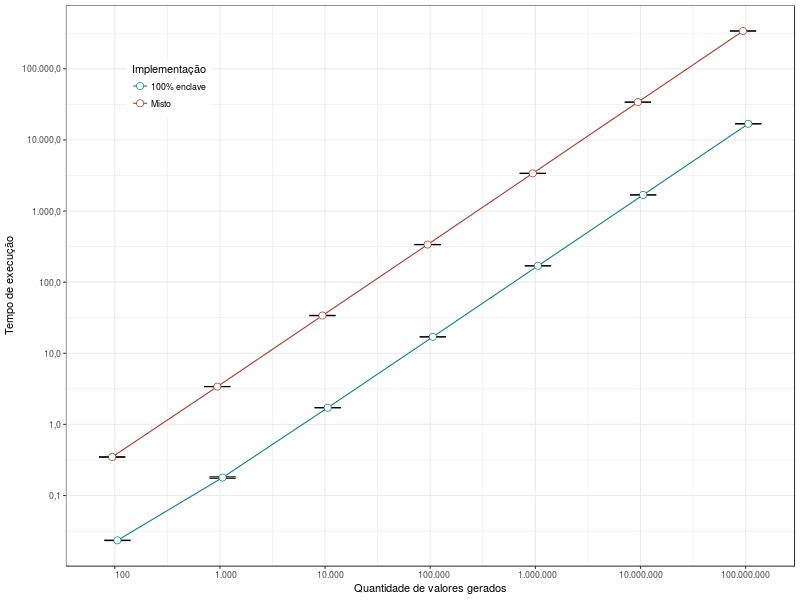
\includegraphics[width=5in]{img/particionamento-aplicacoes-final}
    \caption{Tempos médios para gerar e calcular a soma de $N$ elementos,
    variando $N$ entre, 100 e 100000000, com um intervalo de 95\% de confiança.}
    \label{fig:abordagem_particionamento_aplicacoes}
\end{figure}

\subsection*{Discussão}

A recomendação feita pela Intel, em relação ao particionamento de aplicações, é
de que o enclave contenha apenas o código das funções que lidam diretamente com
dados sensíveis, com o objetivo de manter o TCB o menor possível. Considerando
os resultados obtidos neste experimento, porém, podemos notar que nem sempre
esta divisão será viável, devido à grande sobrecarga gerada no tempo de execução
da aplicação. Esta sobrecarga acontece pelo fato de que, a cada execução de uma
OCall, o processador precisa realizar uma troca de contexto do modo enclave para
o modo normal, e de volta para o modo enclave ao terminar a execução da OCall.
Desta forma, recomendamos que funções da parte insegura que têm muita interação
com funções do enclave da aplicação também sejam implementadas e executadas
dentro do enclave.

% \section{Colocação de aplicações}
% \label{sec:abordagem_colocacao_aplicacoes}

% Na grande maioria das vezes, várias aplicações são executadas simultaneamente em
% um mesmo \textit{host}. Nestas condições, tais aplicações disputam os recursos
% disponíveis na máquina. \fixme{Continua...}

% \subsection*{Experimentos}

% \fixme{Usar o stress}\footnote{\url{http://www.nanoshots.com.br/2016/03/stress-realizando-testes-de-estresse-de.html}}

% \subsection*{Resultados obtidos}

% \subsection*{Discussão}

% \section{Primitivas criptográficas}
% \label{sec:abordagem_primitivas_cripto}

% Como parte da solução SGX, são disponibilizadas diferentes implementações de
% primitivas criptográficas. \fixme{Continua...}

% \subsection*{Experimentos}

% \subsection*{Resultados obtidos}

% \subsection*{Discussão}
\chapter{DynSGX}
\label{chapter:dynsgx}

\section{Introdução}
\label{sec:dynsgx_intro}

Considerando as limitações do SGX apresentadas na Seção~\ref{sec:sgx_limitacoes}
% e as observações feitas nas Seções~\ref{sec:abordagem_particionamento_aplicacoes}
e as observações feitas na Seção~\ref{sec:abordagem_gerencia_memoria}, foi desenvolvida uma ferramenta chamada
DynSGX~\cite{DynSGXCloudCom2017}. DynSGX tem como objetivos: ($i$) permitir o
carregamento e remoção de código dinamicamente em enclaves SGX, ($ii$) garantir
a segurança e privacidade de código, ($iii$) permitir uma melhor gerência de
memória por parte do desenvolvedor e usuário de aplicações SGX, e ($iv$)
facilitar o uso de Intel SGX por desenvolvedores sem conhecimento sobre
programação de aplicações SGX.

DynSGX permite que aplicações seguras sejam inicializadas com enclaves pequenos,
e carregar e remover funções no enclave em tempo de execução, à medida que elas
são necessárias. Isso permite que desenvolvedores e usuários possam gerenciar de
forma melhor o consumo de memória. Além disso, DynSGX faz uso do processo de
atestação remota para estabelecer um canal de comunicação confiável para ser
usado no carregamento e remoção de funções do seu enclave, possibilitando a
privacidade do código das funções.

\section{Componentes}
\label{sec:dynsgx_componentes}

O DynSGX é construído baseado em apenas dois componentes: ($i$) o \texttt{DynSGX
enclave} e ($ii$) o \texttt{DynSGX Client}. O \texttt{DynSGX enclave} funciona
como um TEE, responsável pela segurança e privacidade de código e dados de
desenvolvedores e usuários. O \texttt{DynSGX Client}, por sua vez, funciona como
uma interface entre o \texttt{DynSGX enclave} e seus desenvolvedore de
aplicações e usuários. Outra função do \texttt{DynSGX Client} é automatizar o
processo de conversão de uma aplicação qualquer para uma aplicação segura.
O funcionamento de ambos os componentes é melhor definido nas seções que seguem.

\section{TCB do DynSGX}
\label{sec:dynsgx_tcb}

No \texttt{DynSGX enclave} o TCB é limitado ao Intel SGX SDK e PSW, como
qualquer aplicação SGX, acrescentando-se apenas um conjunto de seis funções
compatíveis com SGX, resultando em um enclave com tamanho inicial de apenas
$1.4\ MB$. Tais funções são usadas para ($i$) realizar o processo de atestação
remota, ($ii$) carregar funções no enclave, ($iii$) executar funções carregadas
dinamicamente, e ($iv$) remover funções do enclave.

Para o processo de atestação remota, apenas a função \textit{enclave\_ra\_init}
precisa ser inserida no enclave. Esta função internamente executa a função
\textit{sgx\_ra\_init} do SDK, que inicia o processo de atestação. Para
carregar funções no enclave, duas funções são necessárias: \textit
{enclave\_get\_fas}, responsável por prover uma lista de funções que já estão
disponíveis no enclave, e \textit{enclave\_register\_function}, responsável por
carregar novas funções no enclave. A função \textit{enclave\_execute\_function}
é utilizada para executar funções carregadas no enclave. Por fim, as funções
\textit{enclave\_unregister\_function} e \textit{enclave\_clear\_functions}
podem ser utilizadas para remover funções do enclave.

O \texttt{DynSGX Client} não é considerado como parte do TCB do DynSGX. Isso
porque ele é um \textit{script} escrito em Python, contendo apenas cerca de $300$
linhas de código, que é executado no ambiente do próprio usuário, podendo ser
facilmente auditado pelo mesmo.

\section{Modelo de programação}
\label{sec:dynsgx_modelo_programacao}

Assim como várias outras ferramentas baseadas em programação na nuvem, DynSGX
segue o modelo cliente-servidor, onde o enclave do DynSGX executa no lado do
servidor, e os desenvolvedores e usuários interagem com ele a partir do lado do
cliente.

DynSGX não requer que desenvolvedores tenham conhecimento sobre como desenvolver
aplicações SGX. Ao invés disso, desenvolvedores podem escrever suas funções como
se estivessem desenvolvendo um programa qualquer na linguagem de programação C.
Após escrever suas funções, uma das ferramentas providas pelo DynSGX, \texttt
{bytes\_extractor} compila o arquivo \textit{.c} que contém o código das
funções, e posteriormente recupera os \textit{bytes} que compõem essas funções.
Os \textit{bytes} recuperados pela ferramenta são então enviados de forma segura
para o enclave do DynSGX, onde são armazenados para uma posterior execução. É
importante mencionar que os arquivos \textit{.c} são compilados com a opção
-fPIC, de modo a gerar um código binário independente de posição.

Para exemplificar esse processo, vamos supor que um usuário deseje computar de
forma segura e privada a soma de dois números inteiros. Para isso, o
desenvolvedor da aplicação escreve uma função chamada \textit{sum\_function},
como a descrita no Código Fonte~\ref{lst:sumFunctionC}.

% \noindent\begin{minipage}{.24\textwidth}
\begin{lstlisting}[language=C, label=lst:sumFunctionC, caption={Exemplo de função C para somar dois números inteiros.}]
int sum_function(int a, int b) {
    return a + b;
}
\end{lstlisting}

Após compilar o arquivo \textit{.c} que contém essa função, a ferramenta \texttt
{bytes\_extractor} recupera os \textit{bytes} do código \textit{Assembler} em
arquitetura \textit{x86-64}, como o exibido no Código Fonte~\ref
{lst:sumFunctionASM}, resultando na seguinte \textit{hexstring}:
{\ttfamily \textbackslash x55\textbackslash x48\textbackslash x89\textbackslash
xe5\textbackslash x89\textbackslash x7d\textbackslash xfc\textbackslash
x89\textbackslash x75\textbackslash xf8\textbackslash x8b\textbackslash
x55\textbackslash xfc\textbackslash x8b\textbackslash x45
\textbackslash xf8\textbackslash x01\textbackslash xd0\textbackslash
x5d\textbackslash xc3}.
Esta \textit{hexstring} pode, então, ser carregada no enclave do DynSGX, onde
ela será registrada e armazenada na \textit{heap}, que é uma área de memória
protegida pelo SGX. Quando um usuário precisa executar a sua função, a \textit
{hexstring} será internamente convertida pra um ponteiro de função antes de ser
executada como uma função qualquer.
\begin{lstlisting}[label=lst:sumFunctionASM, caption={Código \textit{Assembler}
correspondente à função \textit{sum\_function}.}]
    push %rbp
    mov  %rsp,%rbp
    mov  %edi,-0x4(%rbp)
    mov  %esi,-0x8(%rbp)
    mov  -0x4(%rbp),%edx
    mov  -0x8(%rbp),%eax
    add  %edx,%eax
    pop  %rbp
    retq
\end{lstlisting}

Quando uma função não é mais necessária para o usuário, ele pode excluí-la do
enclave do DynSGX, de forma a liberar o precioso espaço de memória que está
sendo ocupado com o código. Internamente, o enclave DynSGX executa uma chamada
da função \textit{free}, que efetivamente libera o espaço de memória para a
\textit{heap}. Atualmente este processo ainda é mecânico, demandando que o
usuário requeira a remoção das funções, mas formas de automatizar este processo
podem ser desenvolvidas, conforme discutidas mais à frente.

\section{Ciclo de vida de aplicações}
\label{sec:dynsgx_ciclovida}

Os enclaves do DynSGX são instanciados com um número mínimo de funções, que são
essenciais para o seu funcionamento. Depois que o enclave é instanciado,
desenvolvedores ou usuários podem estabelecer uma conexão para prover suas
funções dinamicamente ao \texttt{DynSGX enclave}. Após enviar suas funções,
usuários podem executá-las dentro do enclave, e até mesmo removê-las
posteriormente. Os passos necessários para completar esse processo estão
ilustrados na Figura~\ref{fig:softwareLifecycle}, e descritos da seguinte forma:

\begin{enumerate}
    \item O \texttt{DynSGX Client} se comunica com o \texttt{DynSGX enclave} e
    realiza o processo de atestação remota para verificar a integridade e
    identidade do enclave, e estabelecer um canal de comunicação seguro entre
    ambos;
    \item O \texttt{DynSGX Client} compila as funções providas pelo
    desenvolvedor em um arquivo \textit{.c}, recupera os \textit{bytes} do
    código \textit{Assembler} gerado usando a ferramenta \texttt
    {bytes\_extractor}, e envia a \textit{hexstring} obtida para o enclave
    através do canal de comunicação seguro. Como resposta, o \texttt{DynSGX
    Client} recebe um identificador das funções carregadas no enclave;
    \item Usando o canal de comunicação seguro, o \texttt{DynSGX Client}
    solicita que o \texttt{DynSGX enclave} execute alguma das funções que foram
    carregadas dinamicamente no enclave, enviando junto à requisição quaisquer
    parâmetros fornecidos pelo usuário. Como resposta, o resultado da execução
    é enviado de volta ao usuário através do \texttt{DynSGX Client};
    \item Por fim, o usuário usa o \texttt{DynSGX Client} para requisitar que o
    \texttt{DynSGX enclave} remova funções que não serão mais utilizadas, de
    forma a liberar espaço na memória.
\end{enumerate}

\begin{figure}
    \centering
    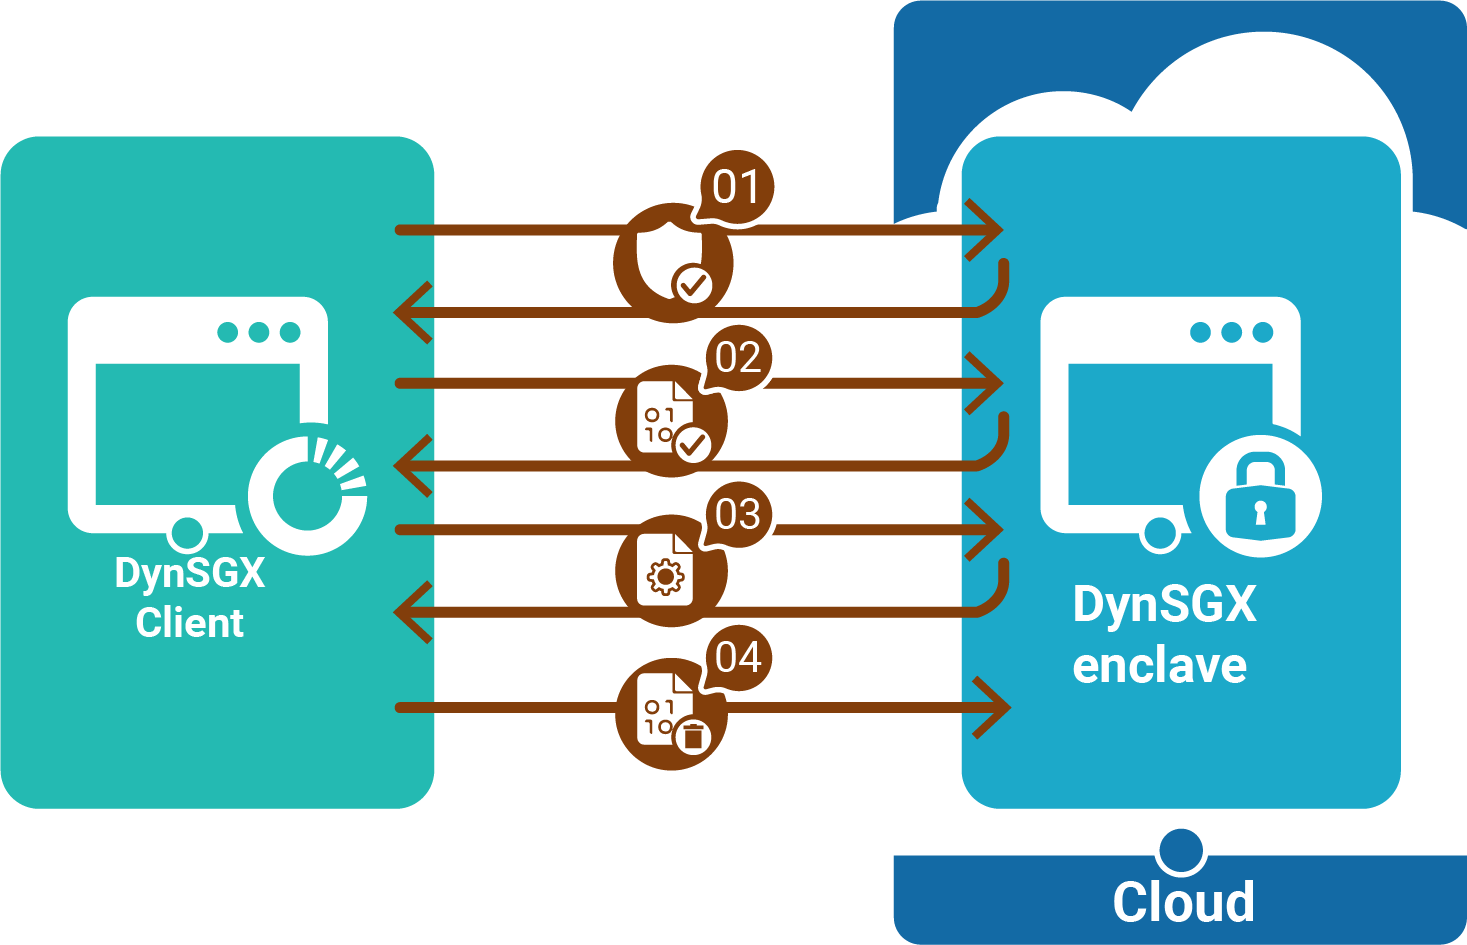
\includegraphics[width=5in]{img/software-lifecycle}
    \caption{Ciclo de Vida de aplicações DynSGX.}
    \label{fig:softwareLifecycle}
\end{figure}

\section{Ligação distribuída de código}
\label{sec:dynsgx_distributed_linking}

Para uma função autocontida, \textit{i.e.}, não utiliza elementos externos,
apenas compilar e enviar os \textit{bytes} da função original é o suficiente.
Entretanto, se a função usar elementos externos, um mecanismo distribuído é
necessário para mapear estes elementos para os seus respectivos endereços no
lado do servidor. Exemplos de elementos externos incluem:
\begin{itemize}
    \item Funções de bibliotecas, como as da \texttt{libc};
    \item Outras funções previamente carregadas no enclave pelo desenvolvedor;
    \item Variáveis globais.
\end{itemize}
DynSGX possui um mecanismo que recupera endereços e tipos de retorno de todas as
funções disponíveis no enclave e os envia para o \texttt{DynSGX Client} na forma
de \textit{JSON}, como o apresentado no Código Fonte~\ref{lst:jsonaddresses},
depois de estabelecido um canal de comunicação seguro pelo processo de atestação
remota.

\begin{lstlisting}[language=C, label=lst:jsonaddresses, caption={Exemplo de
\textit{JSON} contendo o mapeamento de elementos externos para seus respectivos
endereços, que podem ser usados por outras funções.}]
    {
      "snprintf":  "(*(int(*)(0x7f1e438176f0)))",
      "vsnprintf": "(*(int(*)(0x7f1e4381d770)))",
      "strcmp":    "(*(int(*)(0x7f1e438179a0)))",
      ...
    }
\end{lstlisting}

Para uma função como a apresentada no Código Fonte~\ref{lst:func_check_password},
o texto \textit{strcmp}, na linha 3, é substituído por
{\ttfamily (*(int(*)(0x7f1e438179a0)))}. Esse mecanismo funciona por ser o mesmo
que converter e executar um ponteiro de função. O compilador não sabe qual
função estará carregada neste endereço, mas em tempo de execução, a função
\textit{strcmp} estará neste endereço dentro do enclave.

\begin{lstlisting}[language=C, label=lst:func_check_password, caption={Exemplo
de função que usa um elemento externo (a função \textit{strcmp} ).}]
    int check_password(char* input) {
      char password[] = "topsecret123";
      return !strcmp(input, password);
    }
\end{lstlisting}

\section{Requisitos}
\label{sec:dynsgx_requisitos}

Para executar o \texttt{DynSGX enclave} e carregar funções nele em tempo de
execução, três requisitos devem ser satisfeitos:

\begin{itemize}
\item \textbf{\textit{Hardware} com suporte a SGX}: A tecnologia SGX precisa
estar disponível e habilitada no \textit{BIOS}. Tal tipo de \textit{hardware}
está disponível em processadores de prateleira desde o fim de 2015.

\item \textbf{\textit{Driver} SGX}: O \textit{driver} SGX driver precisa estar
instalado, de modo a permitir que o SO e outro conjunto de \textit{software}
seja capaz de acessar o dispositivo.

\item \textbf{SGX PSW}: O SGX PSW\footref{fn:SGXSDK} é usado para instanciar
enclaves SGX, e também para gerar estruturas de dados necessárias durante o
processo de atestação remota. DynSGX requer que uma pequena modificação seja
feita ao PSW. Esta modificação diz respeito à permissão de tornar a \textit
{heap} executável, e pode ser feita aplicando-se um \textit{patch}\footnote
{\url
{https://patch-diff.githubusercontent.com/raw/01org/linux-sgx/pull/63.patch}} ao
código do SGX PSW.
\end{itemize}

\section{Vulnerabilidades}
\label{sec:dynsgx_vulnerabilidades}

Além da vulnerabilidade a ataques de canal lateral inerente do próprio SGX,
DynSGX adiciona uma superfície de ataque: as funções enviadas pelo
desenvolvedor. Para prover suas funcionalidades, DynSGX desabilita duas
proteções: ($i$) canários de pilha nas funções dos desenvolvedores, e ($ii$)
\textit{heap} não executável.

Canários de pilha são usados para detectar um \textit{buffer overflow} antes que
a execução de código malicioso aconteça. Este método funciona inserindo um
número inteiro na memória, cujo valor é escolhido aleatoriamente na
inicialização de um programa, logo antes do ponteiro de retorno da pilha. A
maioria dos ataques de \textit{buffer overflow} sobrescrevem alguns endereços de
memória com o objetivo de sobrescrever o ponteiro de retorno, ganhando assim
controle sobre o processo. Com esse ataque, porém, o valor do canário também é
sobrescrito. Esse valor é verificado para garantir que não foi modificado antes
de uma rotina utilizar o ponteiro de retorno da pilha. Se o valor for
modificado, uma função de erro é executada. Esta função, e sua execução são
adicionadas pelo compilador. Um programador não é capaz de acessá-la nem do lado
do enclave para obter o seu endereço, nem do lado do \texttt{DynSGX Client} para
substituir a sua execução. Portanto, o mecanismo descrito na Seção~\ref
{sec:dynsgx_distributed_linking} não deve funcionar para canários de pilha.

\textit{Heap} não executável é uma medida de segurança que ajuda a prevenir que
certos ataques logrem sucesso, especialmente aqueles que injetam e executam
código na \textit{heap}. Com DynSGX, funções de desenvolvedores são carregadas
dinamicamente para o espaço da \textit{heap}. Portanto, foi necessário
desabilitar esta proteção usando a opção \texttt
{<HeapExecutable>1</HeapExecutable>} no arquivo \texttt{Enclave.config.xml}.

Considerando a limitação do mecanismo ASLR devido ao pequeno espaço de memória,
e desabilitar as proteções de canários de pilha e \textit{heap} não executável,
é extremamente importante um alto empenho no desenvolvimento de código seguro.
O Código Fonte~\ref{lst:func_check_password_vuln1} apresenta um exemplo de
código vulnerável que poderia ser carregado dinamicamente no \textit{DynSGX
enclave}.

\begin{lstlisting}[language=C, label=lst:func_check_password_vuln1, caption=
{Exemplo de função vulnerável a \textit{buffer overflow}.}]
    void check_password(char *input) {
        char buffer[16];
        char password[] = "topsecret123";
        strncpy(buffer, input, strlen(input));
        if (!strcmp(buffer, password))
            access();
    }
\end{lstlisting}

Esta função é vulnerável a \textit{buffer overflow}. Se um atacante prover uma
entrada maior que 16 \textit{bytes}, valores que estivessem armazenados em
memória poderiam ser sobrescritos, como o valor do ponteiro da base da pilha, e
o endereço de retorno. Considerando uma função maliciosa armazenada no endereço
\textit{0x7ffff580160d}, um atacante poderia desviar o fluxo de execução para a
função maliciosa enviando a seguinte carga útil como parâmetro da função:
\textit{AAAAAAAAAAAAAAAAAAAAAAAA\textbackslash x0d
\textbackslash x16\textbackslash x80\textbackslash xf5\textbackslash xff\textbackslash
x7f\textbackslash x00\textbackslash x00}.

Outro exemplo de vulnerabilidade é a formatação não verificada de \textit
{strings}. Uma função de formatação é um tipo especial de função em \textit{C}
que recebe um número variável de argumentos, onde um deles é chamado de formato
de \textit{string}. Sem as devidas precauções neste tipo de função, um atacante
se torna capaz de ler e escrever em qualquer lugar da memória. O Código
Fonte~\ref{lst:func_check_password_vuln2} exemplifica um código vulnerável a
este tipo de ataque.

\begin{lstlisting}[language=C, label=lst:func_check_password_vuln2, caption=
{Exemplo de função vulnerável a formatação não verificada de \textit{strings}.}]
void check_password(char *input) {
    char password[] = "topsecret123";
    if (!strcmp(input, password)) {
        access();
    } else {
        char error[30];
        snprintf(error, 30, input);
        strncat(error, " is incorrect!", 14);
        log_msg(error);
    }
}
\end{lstlisting}

Em uma situação normal, esta função teria o mesmo comportamento da função
apresentada no Código Fonte~\ref{lst:func_check_password}, acrescentando apenas
a funcionalidade de registrar uma mensagem de erro. A vulnerabilidade de
formatação não verificada de \textit{strings} se encontra na linha 7, e um
atacante poderia enviar a seguinte carga útil como parâmetro da função:
{\ttfamily \%10\$p \%11\$p}. Desta forma, a função irá registrar a mensagem:
{\ttfamily 0x6572636573706f74 0x33323174 is incorrect!}. Os numeros apresentados
em hexadecimal são a representação no formato \textit{little endian} da senha.

Dadas as limitações nas proteções de segurança, é muito importante que a escrita
de código seja feita de forma cuidadosa, e regularmente fazer revisões de código.
O uso de ferramentas que examinam o código fonte e alertam sobre possíveis
vulnerabilidades também pode ser útil. Flawfinder\footnote{\url
{https://www.dwheeler.com/flawfinder/}}, Cppcheck\footnote{\url
{http://cppcheck.sourceforge.net/}} e CheckConfigMX~\cite{braz2016} são exemplos
de ferramentas de análise estática de código que podem ser integradas ao DynSGX
para rapidamente encontrar e eliminar potenciais falhas de segurança de funções
antes de enviá-las para o enclave.

\section{Avaliação}
\label{sec:dynsgx_avaliacao}

Para avaliar a performance de aplicações que usam DynSGX, uma série de
experimentos foram realizados, comparando implementações DynSGX com
implementações em C puro e usando SGX. Nesta seção são descritos os experimentos
realizados, e é apresentada uma discussão baseada nos resultados obtidos.

\subsection{Preparação dos experimentos}
\label{subsec:dynsgx_avaliacao_exp_setup}

Os experimentos foram conduzido em uma máquina com sistema operacional Ubuntu
Linux 16.04, um processador Intel i7-6700, e $8\ GB$ de memória principal
disponível. O \texttt{DynSGX enclave} foi desenvolvido na linguagem de
programação \textit{C++}, e o \texttt{DynSGX Client} foi desenvolvido usando a
linguagem de programação \textit{Python} 2.7.

Nos experimentos, foi computada a latência, que representa o tempo total
decorrido desde o início de uma requisição feita pelo cliente para executar uma
função do lado servidor, até o mesmo cliente obter o resultado do processamento
feito. No cálculo da latência também é incluído o tempo para realizar o processo
de atestação remota quando ela é necessária, e de cifrar e decifrar os dados em
ambos os lados para aumentar os níveis de segurança e privacidade dos dados
enviados entre cliente e servidor.

A latência foi calculada baseada em duas funções com comportamentos distintos.
A primeira é a função \textit{sum\_array}, que itera sobre um \textit{array} de
números inteiros, computando a soma de todos eles. A segunda é a função \textit
{recursive\_fibonacci}, que recursivamente calcula o $n$-ésimo termo da sequência
de Fibonacci. Estas duas funções foram escolhidas para ilustrar uma aplicação
com gargalo no consumo de memória, que é uma limitação conhecida do SGX, e uma
aplicação com gargalo no consumo de \textit{CPU}. 

Para avaliar a performance da ferramenta proposta, ambas as funções foram
implementadas de três maneiras distintas. A primeira implementação, feita em
C puro, não provê nenhuma funcionalidade de segurança e privacidade. A segunda
usa o modelo de programação SGX, provendo segurança e privacidade dos dados
envolvidos. A terceira usa o modelo de programação DynSGX, que permite uma
gerência da memória consumida pelas funções de um enclave, e adiciona a
funcionalidade de privacidade do código sendo executado no enclave. Para as
implementações do modelo SGX e DynSGX, foram consirados ambos os casos quando o
processo de atestação remota precisaria ser realizado para estabelecer o canal
de comunicação seguro, e quando este canal já havia sido estabelecido
anteriormente.

\subsection{Experimentos}
\label{subsec:dynsgx_avaliacao_experimentos}

\begin{figure*}
    \centering
    \subfloat[Latência para a função \textit{sum\_array}]
    {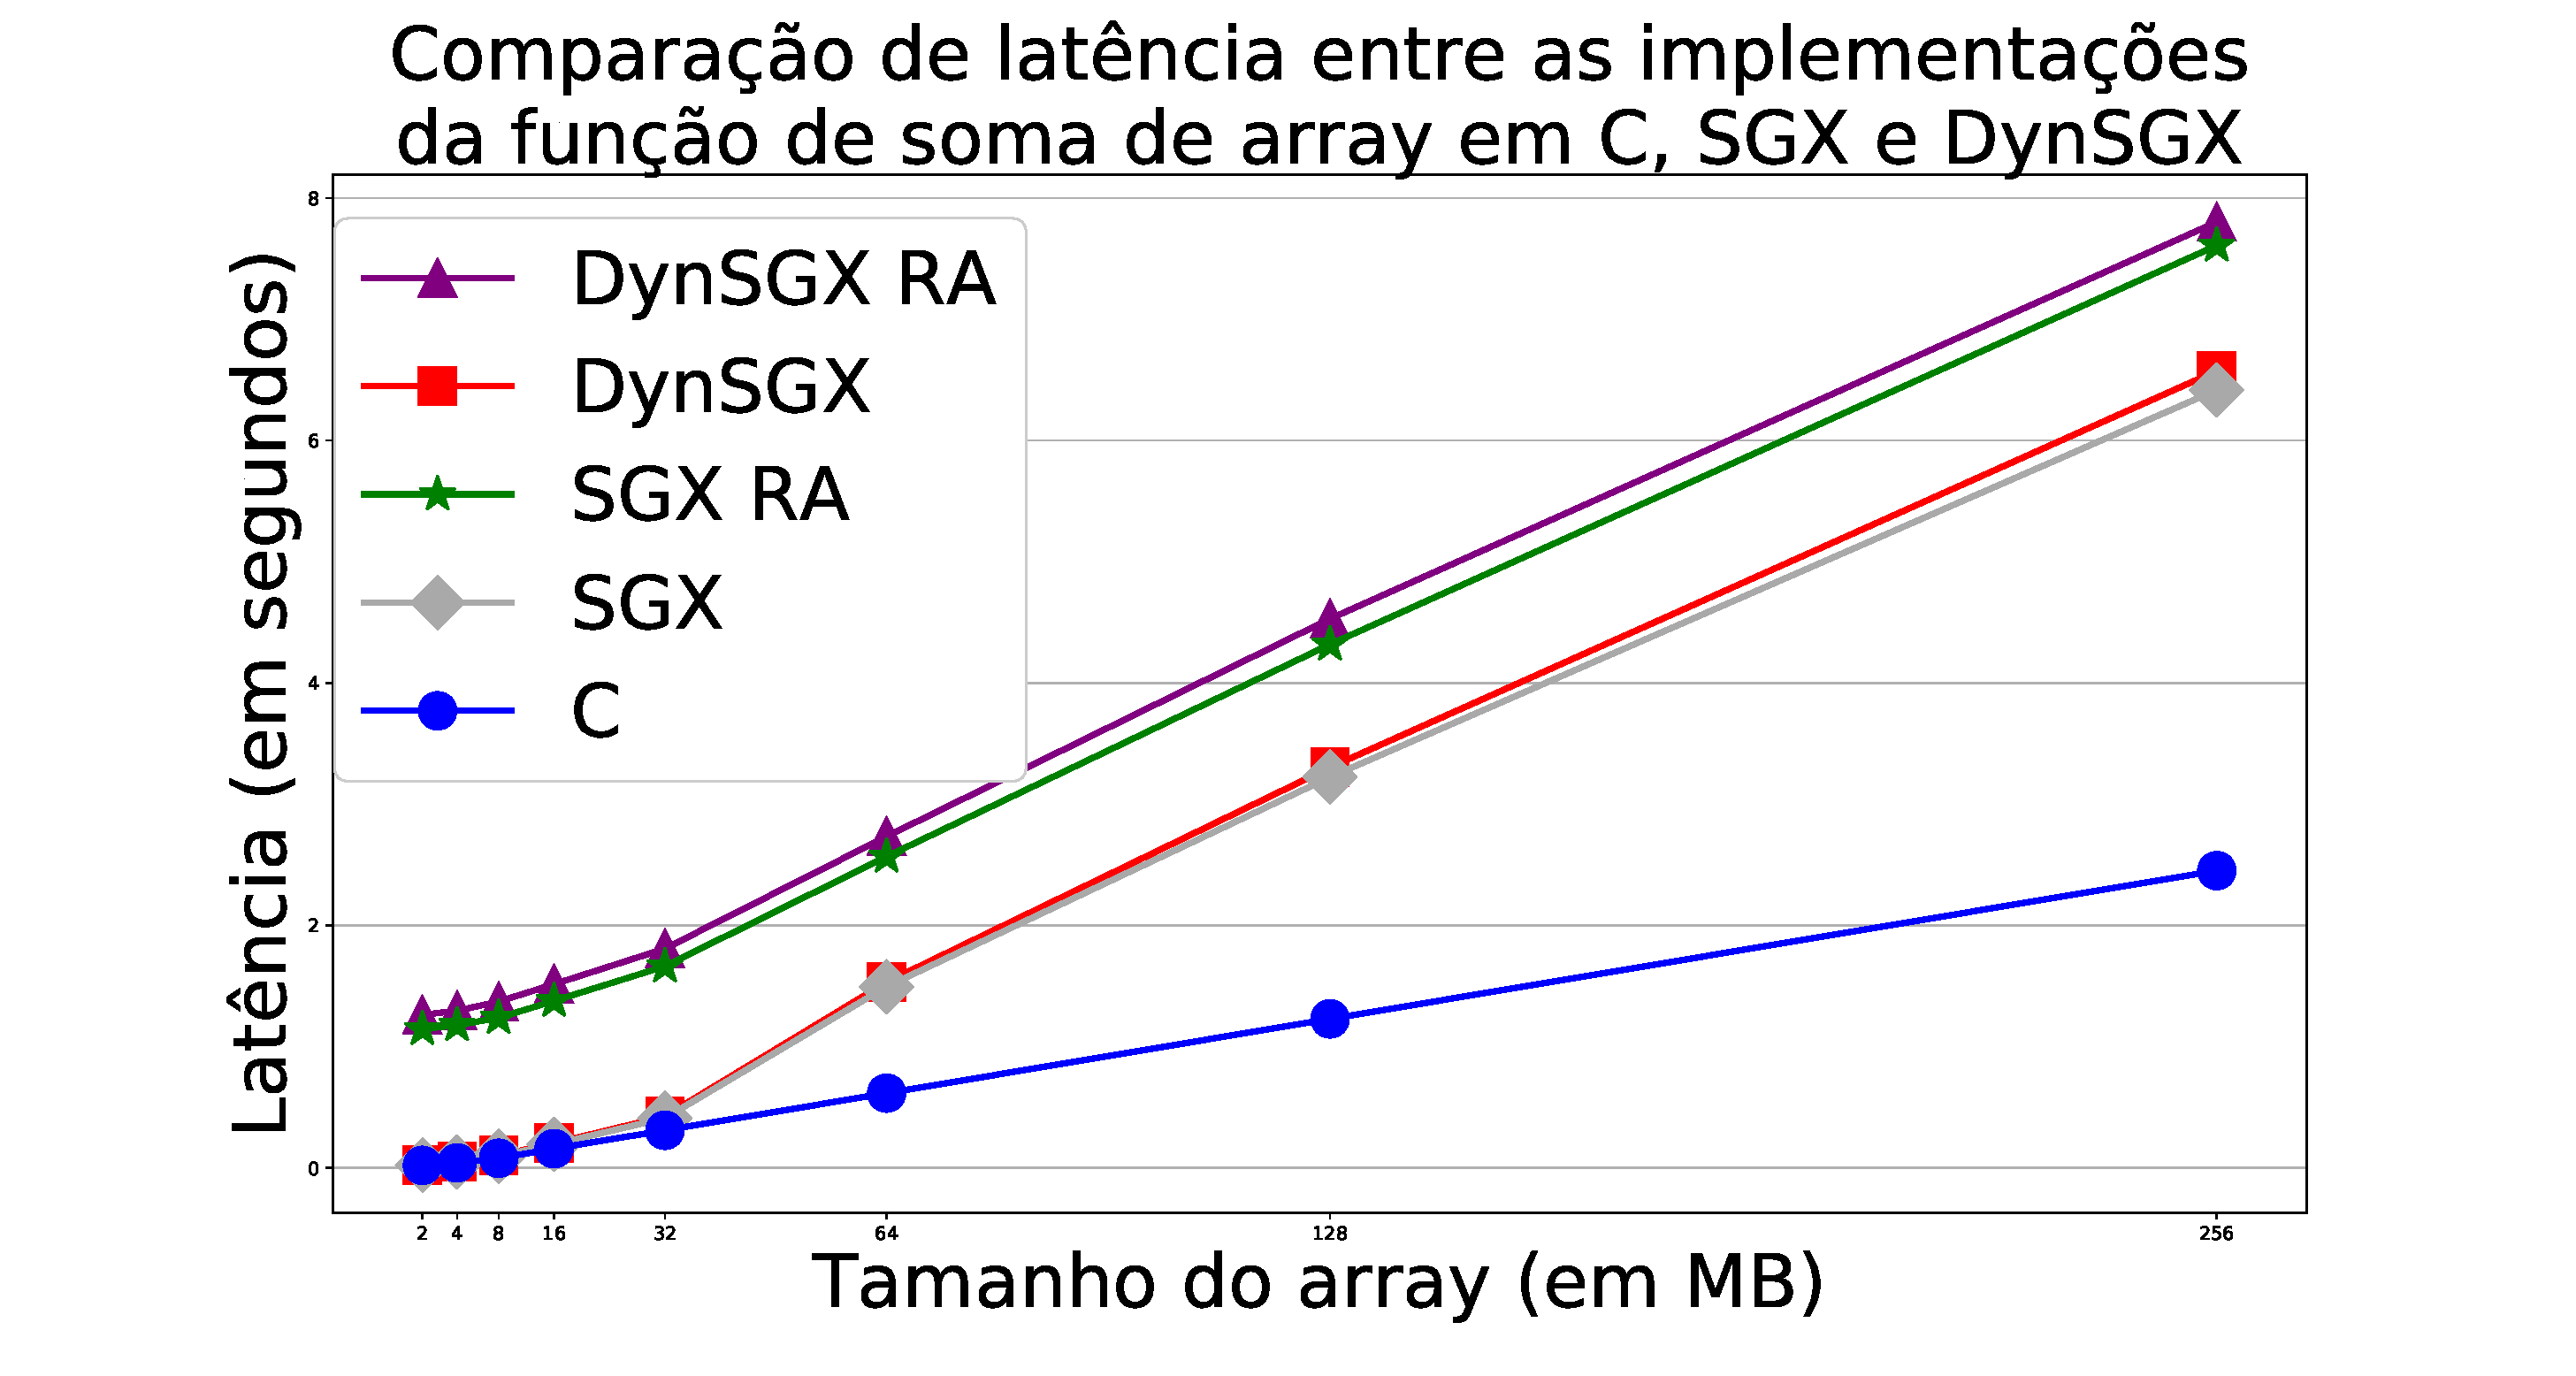
\includegraphics[width=5in]{img/sum_results}
    \label{fig:sum_results}}
    \hfil
    \subfloat[Latência para a função \textit{recursive\_fibonacci}]
    {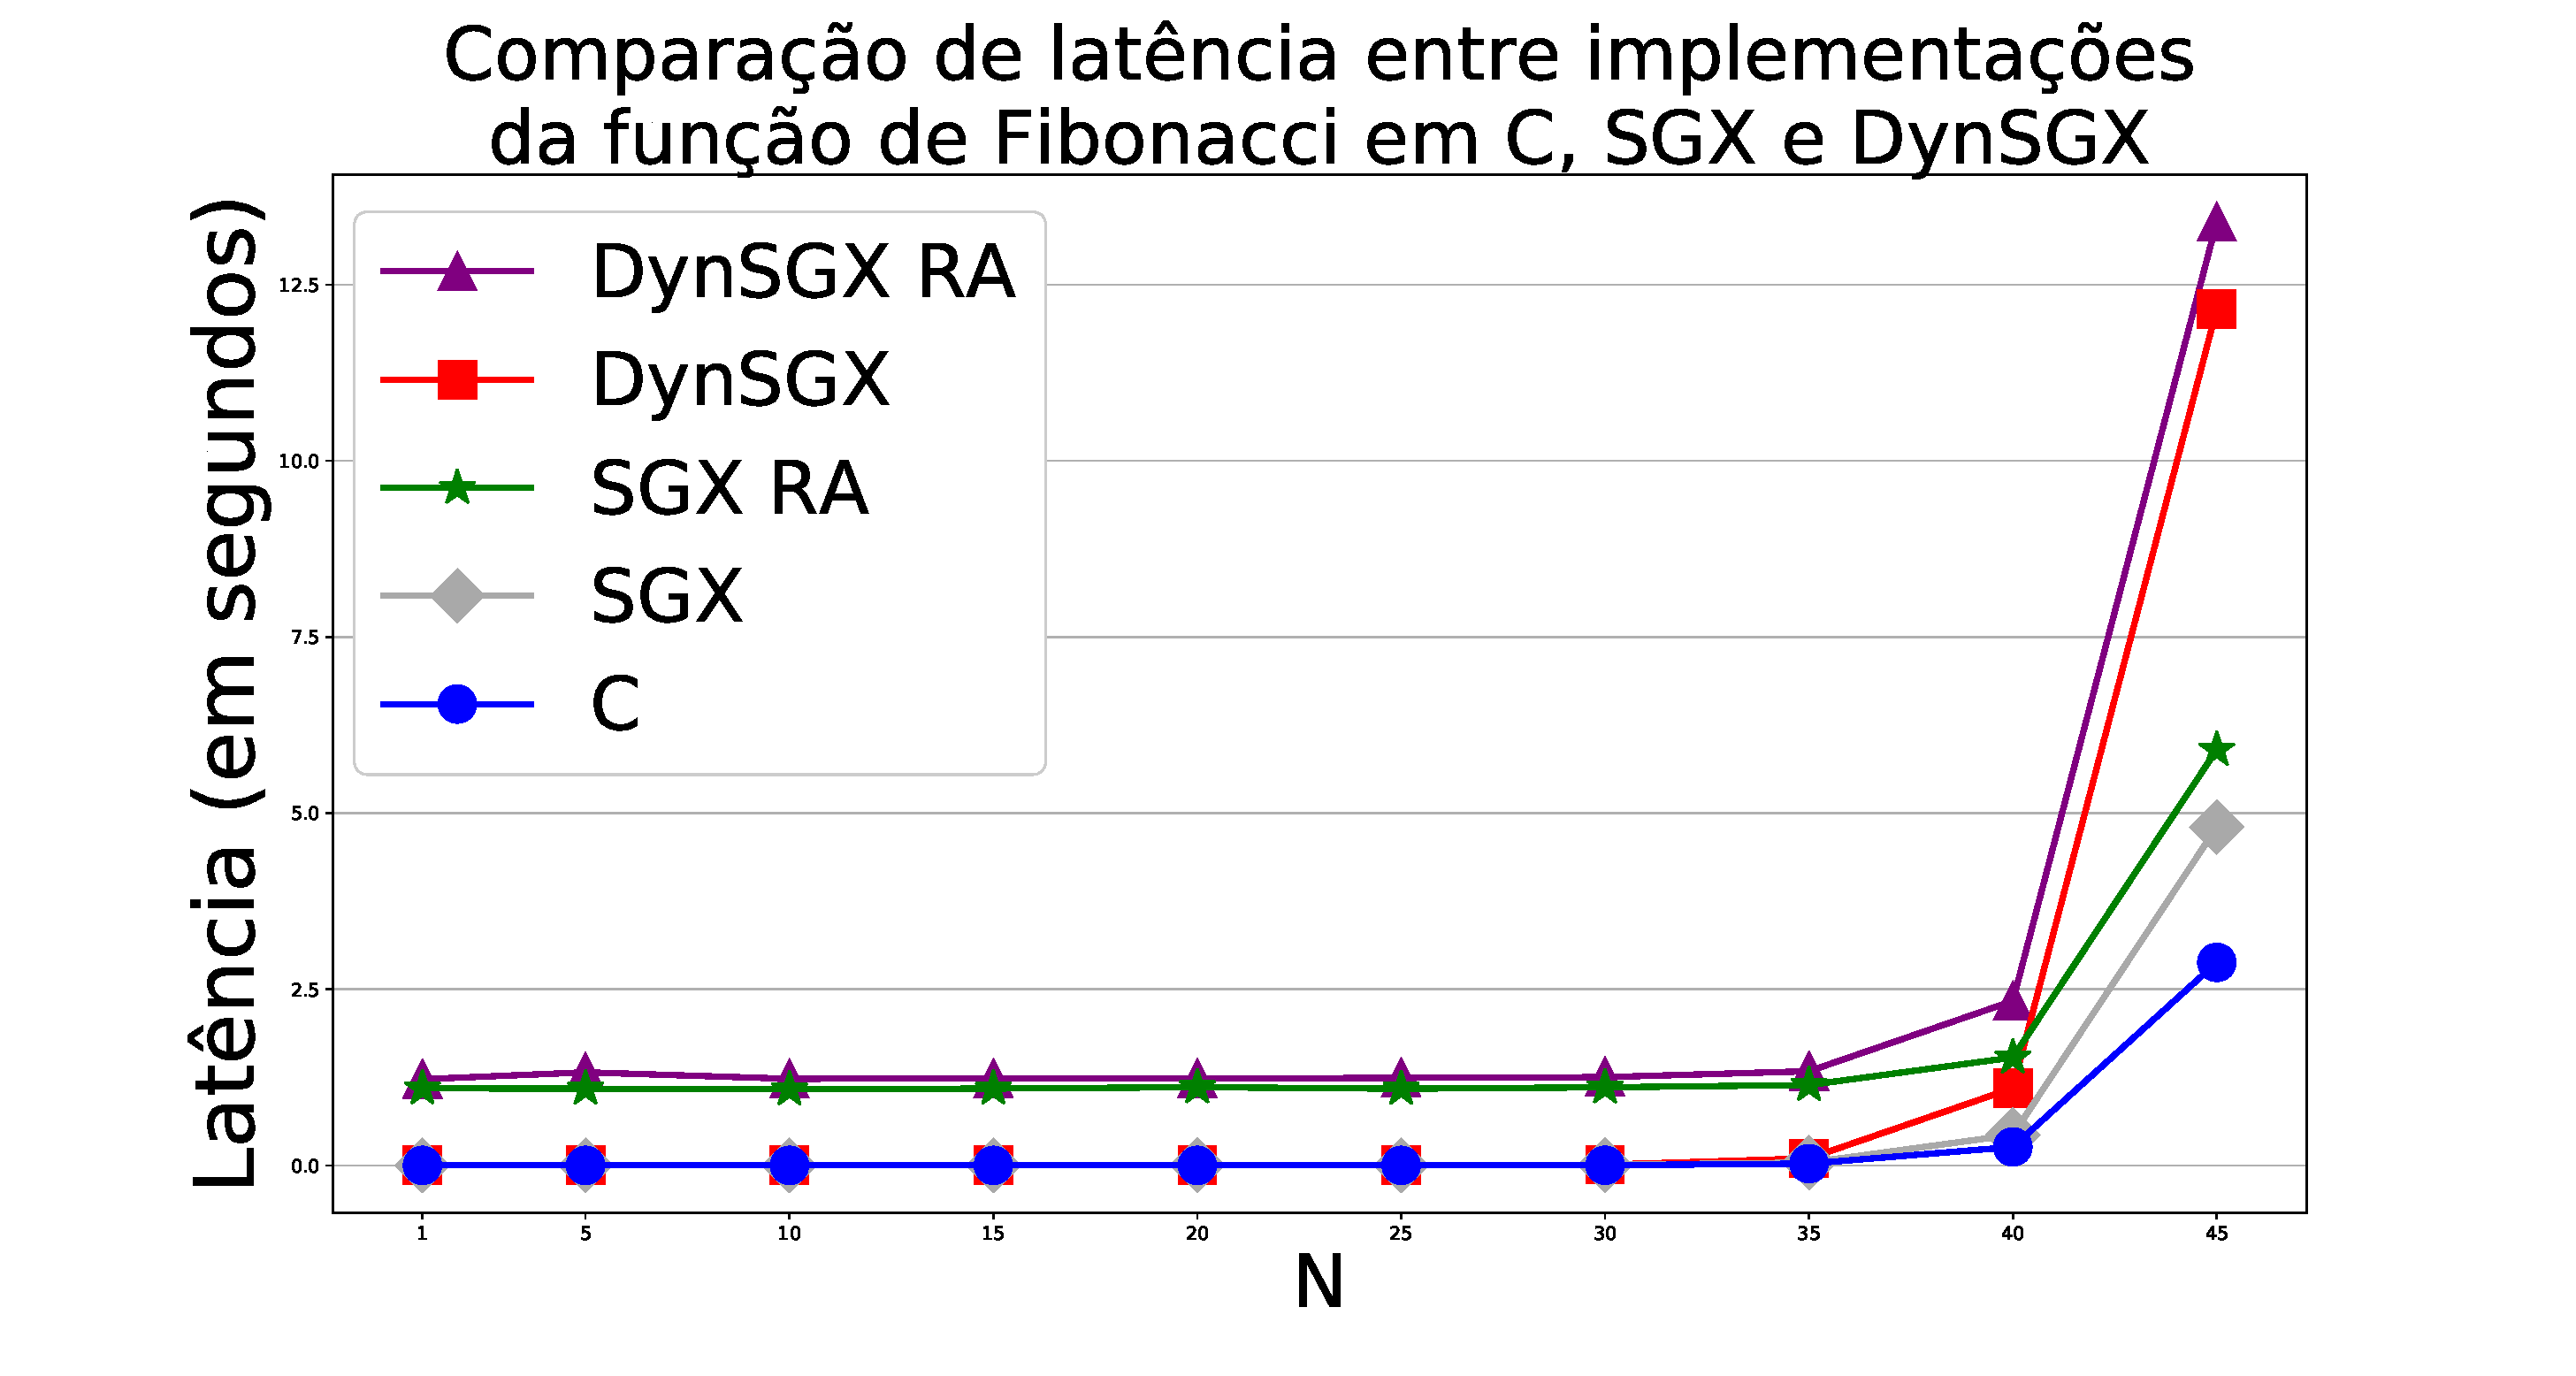
\includegraphics[width=5in]{img/fib_results}
    \label{fig:fib_results}}
    \caption{Comparação de latência entre as implementações em C puro, Intel
    SGX, e DynSGX}
    \label{fig:exp_results}
\end{figure*}

Os experimentos foram constituídos de duas partes. A primeira parte buscava
comparar a latência para computar a função \textit{sum\_array} para \textit
{arrays} com tamanhos de $2$, $4$, $8$, $16$, $32$, $64$, $128$, e $256\ MB$.
A Figura~\ref{fig:sum_results} mostra a mediana dos valores de latência obtidos
nesta parte do experimento. Este experimento serve para nos mostrar o
comportamento do uso de DynSGX com funções iterativas, especialmente quando há
um consumo de memória que extrapola a memória disponível na EPC.

A segunda parte do experimento visa comparar a latência para computar a função
\textit{recursive\_fibonacci} assumindo os valores de $1$, $5$, $10$, $15$,
$20$, $25$, $30$, $35$, $40$, e $45$ para a variável $n$. A Figura~\ref
{fig:fib_results} mostra a mediana dos valores de latência obtidos nesta parte
do experimento. Este experimento é importante para mostrar o comportamento do
uso de DynSGX com funções recursivas.

Em ambas as partes do experimento, para cada tamanho de \textit{array} e para
cada valor da variável $n$, 30 repetições foram executadas. Os resultados
obtidos nestes experimentos têm distribuição enviesada. Por este motivo,
escolhemos a mediana como medida de tendência central utilizada na análise feita.

\subsection{Discussão}
\label{subsec:dynsgx_avaliacao_discussao}

Como pode ser visto na Figura~\ref{fig:exp_results}, ambas as implementações que
usam SGX e DynSGX sempre geram uma sobrecarga considerável se comparadas a
implementação em C puro, que não se preocupa com segurança e privacidade de
dados do usuário. Esta sobrecarga acontece por dois motivos principais: ($i$) o
tempo necessário para realizar o processo de atestação remota, e ($ii$) a
necessidade de cifrar e decifrar dados constantemente.

A partir dos resultados obtidos nos experimentos, pode-se observar também que
para processar funções iterativas, DynSGX apresenta apenas uma pequena
sobrecarga, de aproximadamente $2,5\%$, comparando-se com o uso de SGX.
Este comportamento pode ser observado em ambos os casos quando é necessário
realizar o processo de atestação remota, e quando o canal de comunicação seguro
já foi estabelecido. Neste cenário, nós consideramos os benefícios de usar
DynSGX significantes, por adicionar privacidade do código executado no enclave,
e a possibilidade de gerenciar a memória ocupada por código.

Entretanto, é importante observar que o DynSGX pode não ter uma performance
muito boa no caso de funções recursivas. A Figura~\ref{fig:fib_results} mostra
este cenário, onde o tempo de execução da função \textit{recursive\_fibonacci}
cresce exponencialmente à medida que o número de chamadas recursivas cresce.
Neste cenário, DynSGX tem uma performance muito inferior à performance do SGX.
Este comportamento acontece porque com o DynSGX o código das funções reside na
\textit{heap}, que é um segmento de dados, e compete com outras áreas de dados,
como os quadros de dados das chamadas recursivas, por espaço na \textit{cache} 
do processador. Processadores modernos têm \textit{caches} distintas para código
e dados. Deste modo, a implementação SGX tem melhor performance neste cenário
por manter o código da função na \textit{cache} de instruções.
Este comportamento não é limitado ao DynSGX. Uma implementação C pura ou SGX de
um algoritmo recursivo que armazene código na \textit{heap} também obterá alguma
sobrecarga.

Em relação aos aspectos de segurança mencionados na Seção~\ref
{sec:dynsgx_vulnerabilidades}, é importante evidenciar que desabilitar os
canários de pilha e habilitar a execução da \textit{heap} não necessariamente
implicam riscos para o dono do \textit{hardware} executando o \texttt{DynSGX
enclave}, uma vez que em ambientes de computação na nuvem é possível configurar
outras camadas de segurança. Por exemplo, o \texttt{DynSGX enclave} poderia ser
executado em um ambiente isolado como uma máquina virtual.

Por fim, na Tabela~\ref{tab:dynsgx_sgx_comparison} é apresentada uma comparação
das vantagens e desvantagens de cada uma das três implementações consideradas
nos experimentos.

\begin{center}
    \begin{table}
        \caption{Comparação de performance entre as implementações em C puro,
        SGX e DynSGX}
        \label{tab:dynsgx_sgx_comparison}
        \centering
        \begin{tabular}{|c|c|c|c|c|c|c|}
            \cline{2-7}
            \multicolumn{1}{ c |}{} & \multicolumn{2}{ c |}{\textbf{Segurança}} & \multicolumn{2}{ c| }{\textbf{Privacidade}} & \multicolumn{2}{ c |}{\textbf{Performance}} \\ \cline{1-7}
            \textbf{Impl.} & \textbf{dados} & \textbf{código} & \textbf{dados} & \textbf{código} & \textbf{iterativo} & \textbf{recursivo} \\ \hline
            C puro &  &  &  &  & Alta & Alta \\ \hline
            SGX & \ding{51} & \ding{51} & \ding{51} &  & Média & Média \\ \hline
            DynSGX & \ding{51} & \ding{51} & \ding{51} & \ding{51} & Média & Baixa \\ \hline
        \end{tabular}
    \end{table}
\end{center}

\section{Considerações}
\label{sec:dynsgx_consideracoes}

As limitações existentes na tecnologia Intel SGX levou à construção da
ferramenta DynSGX, apresentada neste capítulo. A ferramenta proposta facilita o
desenvolvimento de aplicações que fazem uso de SGX, uma vez que não requer que o
desenvolvedor adquira conhecimento sobre as APIs da tecnologia. A ferramenta
também possibilita a gerência de memória ocupada pelo código de uma aplicação, o
que não era possível no modelo de programação convencional do SGX.

Considerando a avaliação conduzida sobre a ferramenta, foi mostrado que a
ferramenta possibilita obter privacidade também do código da aplicação a ser
executada dentro do enclave, gerando apenas uma pequena sobrecarga em relação a
aplicações SGX comuns em alguns casos.

Por fim, é necessário ressaltar que DynSGX não deve ser aplicado em todos os
cenários. Um dos cenários que se mostrou impróprio para o uso de DynSGX é o das
funções recursivas que possuem uma quantidade exponencial de chamadas recursivas.
Neste caso, o desenvolvedor deve analisar se o custo decorrente do uso do DynSGX
é justificado pelos ganhos de privacidade do código e gerenciamento de memória
consumida por código.
\chapter{Conclusão}
\label{chapter:conclusao}

Neste capítulo, apresentamos, na Seção~\ref{sec:conclusao_sumario}, um sumário
do que foi proposto e realizado nesta pesquisa. Além disso, apresentamos algumas
considerações sobre as análises feitas, bem como sobre a ferramenta proposta no
Capítulo~\ref{chapter:dynsgx}. Por fim, na Seção~\ref
{sec:conclusao_limitacoes_trabalhos_futuros}, apresentamos as limitações deste
trabalho, e possíveis trabalhos futuros.

\section{Sumário}
\label{sec:conclusao_sumario}

Nesta pesquisa de mestrado discutimos os principais desafios no desenvolvimento
de aplicações com propriedades de segurança e privacidade de dados, usando a
tecnologia Intel SGX. Para tanto, no Capítulo~\ref{chapter:abordagem}, 
analisamos como várias decisões na implementação e no uso de aplicações SGX
influenciam no seu desempenho geral, e nas garantias de segurança realacionadas
ao tamanho do TCB da aplicação. As características analisadas incluem como
devemos gerenciar a memória de enclaves SGX, como deve ser o particionamento
entre parte segura e parte insegura das aplicações SGX, e como deve ser o
particionamento dos dados a serem processados dentro de enclaves SGX.

As análises apresentadas servem para auxiliar desenvolvedores na tomada de
decisões sobre boas práticas a serem aplicadas na arquitetura de aplicações
seguras, diferenciando-se no particionamento de código e dados, e gerência de
memória de tais aplicações em comparação a aplicações inseguras, onde esses
aspectos não têm tanto impacto.

Este trabalho foi motivado pela crescente popularidade do uso da tecnologia
Intel SGX para desenvolver aplicações que proveem segurança e privacidade de
dados, observada na literatura, e pela falta da definição de padrões no
desenvolvimento de tais aplicações, a não ser as recomendações feitas pela
própria Intel. Em experimentos realizados em nosso ambiente, constatamos que o
mau planejamento de uma aplicação SGX pode acarretar uma grande perda de
desempenho da mesma, chegando a um custo de execução até $534\%$ mais alto,
comparado a aplicações bem planejadas.

Considerando as análises feitas, propomos uma ferramenta, DynSGX, que serve
como uma alternativa ao modelo de programação do Intel SGX, facilitando o uso
desta tecnologia, \textit{i.e.}, não requer que o desenvolvedor conheça o SGX
SDK, e o gerenciamento de memória de suas aplicações SGX. Nós avaliamos esta
ferramenta, por meio de experimentos, comparando o seu desempenho com o
desempenho de uma aplicação desenvolvida usando o modelo de programação
tradicional do Intel SGX. Os resultados obtidos nos experimentos indicam que
o DynSGX pode ser utilizado de forma eficiente para o processamento de funções
iterativas, gerando uma sobrecarga de apenas $2,5\%$ em relação ao uso de SGX
puro, porém o seu uso para processamento de funções recursivas pode ter
uma performance muito inferior à solução que usa SGX puro. 

\section{Limitações e trabalhos futuros}
\label{sec:conclusao_limitacoes_trabalhos_futuros}

Apesar de mostrar algumas das características de aplicações SGX que afetam o seu
desempenho, a lista aqui apresentada não é exaustiva, e não considera como duas
ou mais características em conjunto podem impactar no desempenho das aplicações.
Desta forma, mais análises precisam ser feitas para determinar outras boas
práticas a serem aplicadas no desenvolvimento de aplicações SGX.

A segunda limitação deste trabalho está na forma como foi avaliada a segurança
das aplicações, onde apenas foi considerado o tamanho do TCB.

Uma outra limitação deste trabalho diz respeito à ferramenta proposta, DynSGX.
O DynSGX foi desenvolvido com o intuito de funcionar como uma plataforma de
função como um serviço (FaaS, do inglês \textit{Function as a Service}). A sua
implementação atual, porém, requer que ambos o desenvolvedor e o usuário das
funções carregadas no \texttt{DynSGX enclave} sejam a mesma pessoa, de modo a
ganhar confiança em relação a segurança e privacidade dos dados processados.
Além disso, como citado anteriormente, a tarefa de remover funções do enclave do
DynSGX é demasiadamente mecanizada. A automatização desta tarefa deve ser
tratada em uma futura versão do DynSGX.

Como possíveis trabalhos futuros, além de solucionar as limitações destacadas,
propomos a evolução do DynSGX, de forma a transformá-lo em uma plataforma
completa de aplicações \textit{serverless}, possibilitando o desenvolvimento e
uso de aplicações por pessoas diferentes, com garantias de segurança e
privacidade de dados e código carregados na plataforma. Essa abordagem permite
maiores facilidade e segurança no desenvolvimento de aplicações SGX, bem como um
melhor gerenciamento automático de memória utilizada pelos enclaves do DynSGX.

%%%%%%%%%%%%%%%%%%%%%%%%%%%%%%%%%%%%%%%%%%%%%%%%%%%%%%%%%%%%%%%%%%%%%%%%%%%%%%%%
%% BIbliografia
%% Coloque suas referencias no arquivo ref.bib e descomente as proximas duas linhas

\bibliographystyle{alpha} % estilo de bibliografia   plain,unsrt,alpha,abbrv.
\bibliography{bib/ref} % arquivos com as entradas bib.

%%%%%%%%%%%%%%%%%%%%%%%%%%%%%%%%%%%%%%%%%%%%%%%%%%%%%%%%%%%%%%%%%%%%%%%%%%%%%%%%
%% Apendice
% Caso seja necessario algum apendice, descomente a proxima linha.

\appendix
\chapter{Exemplo de aplicação SGX}
\label{appendix:aplicacao_sgx}

Como discutido na Seção~\ref{sec:sgx_modelo_programacao}, aplicações SGX são
divididas entre parte segura, que executa dentro de enclaves SGX, e parte
insegura, usada para instanciar o enclave da aplicação, executar ações que não
necessitem de garantias de segurança, e intermediar qualquer tipo decomunicação
entre um enclave e o mundo externo a ele, inclusive a execução de \textit
{system calls}. Além disso, precisamos definir uma interface de comunicação
entre as partes segura e insegura (arquivo EDL).

Para exemplificar o desenvolvimento de aplicações SGX, utilizamos a seguir a
aplicação utilizada nos experimentos da Seção~\ref
{sec:abordagem_particionamento_dados}.

\section{Desenvolvimento do arquivo EDL}
\label{sec:appendix_aplicacao_sgx_arquivo_edl}

A primeira coisa a se pensar no desenvolvimento de aplicações SGX é em como
particionar a aplicação entre as partes segura e insegura, e, mais precisamente,
é necessário pensar em como ambas as partes se comunicam entre si. Para isso,
precisamos escrever um arquivo EDL, contendo a declaração das ECalls (declaradas
na seção \textit{trusted} do arquivo EDL), e das OCalls (declaradas na seção
\textit{untrusted} do arquivo EDL).

No caso da aplicação em questão, apenas a função \textit{enclave\_sum} cruza
entre as partes segura e insegura. O conteúdo do arquivo EDL está descrito no
Código Fonte~\ref{lst:arquivo_edl}. No código apresentado, o parâmetro "\textit
{in}", entre colchetes, indica que o \textit{array} é um ponteiro de entrada, ou
seja, será copiado da parte insegura para o enclave antes da execução da função
\textit{enclave\_sum}. O parâmetro "\textit{size=array\_size}" indica que o
tamanho do \textit{array}, em \textit{bytes}, é dado pela variável \textit
{array\_size}. 

\begin{lstlisting}[language=C, label=lst:arquivo_edl, caption={Arquivo EDL
contendo a declaração das funções que cruzam a fronteira entre as partes segura
e insegura da aplicação SGX.}]
    // Arquivo enclave.edl
    enclave{
        trusted{
            public long enclave_sum(
                [in, size=array_size] int *array,
                                   size_t  array_size
            );
        };
        untrusted{}; // Nenhuma função a declarar aqui.
    };
\end{lstlisting}

Após a criação do arquivo EDL, utlizamos a ferramenta \textit{sgx\_edger8er} para
compilar o arquivo EDL, e gerar as interfaces de comunicação entre as partes
segura e insegura propriamente ditas. Executamos, portanto, os comandos
\lstinline[breaklines=true,keywordstyle=\ttfamily]!sgx_edger8r --trusted enclave.edl --search-path ${SGXSDK_PATH}/include!
e \lstinline[breaklines=true,keywordstyle=\ttfamily]!sgx_edger8r --untrusted enclave.edl --search-path ${SGXSDK_PATH}/include!,
para gerar os arquivos de interface a serem utilizados, respectivamente, pelas
partes segura e insegura da aplicação.

Mais informações sobre a sintaxe dos arquivos EDL pode ser encontrada no
documento de referência para desenvolvedores~\cite{sgxdeveloperreference}.

\section{Desenvolvimento do enclave}
\label{sec:appendix_aplicacao_sgx_codigo_enclave}

O código do enclave contém a implementação de todas as ECalls declaradas no
arquivo EDL, adicionando-se o código de quaisquer funções internas necessárias.
No caso da aplicação em questão, precisamos escrever apenas a implementação da
função \textit{enclave\_sum}. Tal implementação pode ser encontrada no Código
Fonte~\ref{lst:arquivo_enclave_cpp}.

\newpage
\begin{lstlisting}[language=C, label=lst:arquivo_enclave_cpp, caption={Arquivo
contendo a implementação das funções a serem executadas totalmente dentro do
enclave da aplicação SGX.}]
    // Arquivo enclave.cpp
    #include "stdlib.h"
    #include "enclave_t.h" // Gerado pela ferramenta sgx_edger8er

    long enclave_sum( int *array, size_t array_size) {
        long sum = 0;
        int i;
        for (i=0; i<array_size/sizeof(int); ++i){
            sum += array[i];
        }
        return sum;
    }
\end{lstlisting}

O enclave deve, então, ser compilado com o compilador \textit{g++}, de modo a
gerar uma biblioteca dinâmica (\textit{.so} no caso do Linux, ou \textit{.dll}
no caso do Windows). Por fim, o enclave deve ser assinado usando a ferramenta
\textit{sgx\_signer}, usando o comando
\lstinline[breaklines=true,keywordstyle=\ttfamily]!sgx_signer sign -key priv_key -enclave enclave.so -out enclave.signed.so -config enclave.config.xml!,
onde {\ttfamily priv\_key} é a chave privada do desenvolvedor, {\ttfamily
enclave.so} é a biblioteca dinâmica do enclave produzido pelo \textit
{sgx\_edger8er}, {\ttfamily enclave.signed.so} é o enclave resultante, assinado,
e {\ttfamily enclave.config.xml} é o arquivo de configuração das características
do enclave SGX, conforme exibido no Código Fonte~\ref
{lst:arquivo_enclave_config_xml}.

Entre as configurações do arquivo \textit{enclave.config.xml} que podemos,
destacar, estão o tamanho máximo da \textit{heap} e tamanho máximo da pilha do
enclave. Ambas configurações têm impacto no direto no tempo necessário para a
instanciação de um enclave, pois o SGX aloca todo esse espaço de memória durante
a instanciação do enclave. No caso caso específico da configuração do enclave
utilizada nos experimentos da Seção~\ref{sec:abordagem_particionamento_dados},
a instanciação de um enclave levava cerca de 30 segundos para completar.
Enclaves com tamanhos máximos de \textit{heap} e pilha menores que os usados
nesta configuração levam menos tempo para serem instanciados.

\newpage
\begin{lstlisting}[language=XML, label=lst:arquivo_enclave_config_xml, caption={Arquivo
de configuração do enclave SGX.}]
    // Arquivo enclave.config.xml
    <EnclaveConfiguration>
    <ProdID>0</ProdID>
    <ISVSVN>0</ISVSVN>
    <StackMaxSize>0x8000</StackMaxSize>
    <HeapMaxSize>0x100000000</HeapMaxSize>
    <TCSNum>10</TCSNum>
    <TCSPolicy>1</TCSPolicy>
    <DisableDebug>0</DisableDebug>
    <MiscSelect>0</MiscSelect>
    <MiscMask>0xFFFFFFFF</MiscMask>
</EnclaveConfiguration>
\end{lstlisting}

Mais informações sobre o arquivo de configuração do enclave podem ser
encontradas no documento de referência para desenvolvedores~\cite
{sgxdeveloperreference}.

\section{Desenvolvimento da parte insegura da aplicação}
\label{sec:appendix_aplicacao_sgx_parte_insegura}

A parte insegura de uma aplicação SGX compreende todo o código que lida com
dados não sensíveis, adicionando-se o código necessário para instanciar e se
comunicar com o enclave, e a implementação de quaisquer OCalls que tenham sido
declaradas no arquivo EDL. No caso da aplicação em questão, nenhuma OCall
precisa ser implementada. O código necessário para a parte insegura desta
aplicação, é exibido no Código Fonte~\ref{lst:arquivo_app_cpp}.

O fluxo da aplicação pode ser descrito nos seguintes passos:

\begin{enumerate}
    \item A aplicação instancia o enclave SGX (linhas 13-19);
    \item A aplicação gera um \textit{array} com 1GB, povoado por números
    inteiros aleatórios (linhas 20-22);
    \item A aplicação invoca a função do enclave que calcula a soma dos valores
    contidos em uma partição do \textit{array} (linha 29);
    \item A aplicação soma o resultado obtido do enclave ao total armazenado na
    variável \textit{sum} (linha 30);
    \item A aplicação repete os passos 3 e 4 até que todas as partições do
    \textit{array} tenham sido processadas (linhas 27-31);
    \item A aplicação exibe o resultado da soma de todos os elementos do \textit
    {array} (linha 32);
    \item A aplicação destrói o enclave (linha 33).
\end{enumerate}

\begin{lstlisting}[language=C, label=lst:arquivo_app_cpp, caption={Arquivo
contendo a implementação da parte insegura da aplicação SGX.}]
    // Arquivo app.cpp
    #include "stdlib.h"
    #include "enclave_u.h" // Gerado pela ferramenta sgx_edger8er
    #include "sgx_urts.h" // Necessário para instanciar enclaves

    #define ENCLAVE_NAME "enclave.signed.so"
    #define MB_SIZE 1024*1024
    #define ARRAY_SIZE 4096
    #define CHUNK_SIZE 1

    int main(){

        sgx_enclave_id_t eid;
        sgx_status_t ret = SGX_SUCCESS;
        sgx_launch_token_t launch_token;
        int updated = 0;
        ret = sgx_create_enclave( // Instancia um enclave SGX
                ENCLAVE_NAME, SGX_DEBUG_FLAG, &launch_token,
                &updated, &eid, NULL );
        int total_num_of_elements = ARRAY_SIZE * MB_SIZE / sizeof(int);
        int *array = (int *) calloc(total_num_of_elements,sizeof(int));
        generate_random_numbers(array, total_num_of_elements); // Preenche array com números inteiros aleatórios
        int chunk_num_of_elements = CHUNK_SIZE * MB_SIZE / sizeof(int);
        long sum = 0, partial_sum;
        int i, idx;

        for(i=0; i<total_num_of_elements/chunk_num_of_elements; ++i){
            idx = i*chunk_num_of_elements;
            enclave_sum(eid, &partial_sum, &array[idx], CHUNK_SIZE);
            sum += partial_sum;
        }
        printf("A soma dos elementos do array é: %ld.\n", sum);
        sgx_destroy_enclave(eid);
        return 0;
    }
\end{lstlisting}
%%%%%%%%%%%%%%%%%%%%%%%%%%%%%%%%%%%%%%%%%%%%%%%%%%%%%%%%%%%%%%%%%%%%%%%%%%%%%%%%

\end{document}